\documentclass{seal_thesis}

\thesisType{Master Thesis}
\date{\today}
\title{AmbientTeams}
\subtitle{Staying socially connected in remote knowledge work teams}
\author{Dario Bugmann}
\home{Aarau} % Geburtsort
\country{Switzerland}
\legi{15-708-852}
\prof{Prof. Dr. Thomas Fritz}
\assistent{Dr. André Meyer, Alexander Lill}
\email{dario.bugmann@uzh.ch}
\url{https://github.com/HASEL-UZH/PA.AmbientTeam}
\begindate{15.2.2021}
\enddate{22.7.2021}

\usepackage{subcaption}
\usepackage{float}
\usepackage{hyperref}
\usepackage{cleveref}
\usepackage{enumitem}
\usepackage{booktabs}
\usepackage{multirow}
\usepackage[english]{babel}
\usepackage{csquotes}
\usepackage{tabularx}
\renewcommand{\mkbegdispquote}[2]{\itshape}
\usepackage[toc,page]{appendix}
\usepackage[style=alphabetic]{biblatex}
\addbibresource{thesis.bib}


\usepackage{array}
\usepackage{arydshln}
\setlength\dashlinedash{0.2pt}
\setlength\dashlinegap{1.5pt}
\setlength\arrayrulewidth{0.3pt}

\renewcommand{\arraystretch}{1.1}

\begin{document}
\maketitle

\frontmatter

\begin{acknowledgements}
    I thank Prof. Dr. Thomas Fritz, Dr. André Meyer, and Alexander Lill for the opportunity to write this thesis, the time they took for it, and the constructive feedback they were always able to give me. I thank them for always having an open ear for my thoughts and suggestions. I am very grateful for the beautiful trip to Vitznau where I could meet all the members of the HASE research group. A big thank you to all my study participants who took the time to help me with this project and gave such great feedback. I greatly appreciate my family and friends and am grateful for their support. Last but not least, a special thank you to Nora for all her love and support and the faith she always had in me.
\end{acknowledgements}

\begin{abstract}
    With the switch to telecommuting, informal and spontaneous conversations are less likely to occur due to the absence of important cues from colleagues. The lack of such social interactions can lead to feelings of isolation in the workplace. To this end, we developed AmbientTeams, an unobtrusive and informal tool that seeks to reduce the perceived distance between remote colleagues by creating opportunities for more casual interactions. AmbientTeams attempts to do this by taking a micro-blogging approach that allows moods and status updates to be shared with the team. We evaluated our research prototype on a group of five knowledge workers who used the tool for a week. The results show that participants were more aware of each other's moods and availability status and got to know each other better. In addition, the study showed the potential of AmbientTeams to enable more (natural) communication.
\end{abstract}

\begin{zusammenfassung}
    Mit der Umstellung auf Telearbeit werden informelle und spontane Gespräche weniger wahrscheinlich, da wichtige Hinweise von Kollegen fehlen. Der Mangel an solchen sozialen Interaktionen kann zu Gefühlen der Isolation am Arbeitsplatz führen. Zu diesem Zweck haben wir AmbientTeams entwickelt, ein unaufdringliches und informelles Tool, das die gefühlte Distanz zwischen entfernten Kollegen verringern soll, indem es Möglichkeiten für informellere Interaktionen schafft. AmbientTeams versucht dies, indem es einen Micro-Blogging-Ansatz verfolgt, der es erlaubt, Stimmungen und Status-Updates mit dem Team zu teilen. Unseren Forschungsprototyp haben wir an einer Gruppe von 5 Wissensarbeitern evaluiert, die das Tool eine Woche lang verwendet haben. Die Ergebnisse zeigen, dass die Teilnehmer die Stimmungen und den Verfügbarkeitsstatus der anderen besser wahrnahmen und sich gegenseitig besser kennenlernten. Darüber hinaus zeigte die Studie das Potenzial von AmbientTeams, mehr (natürliche) Kommunikation zu ermöglichen.
\end{zusammenfassung}

\tableofcontents
\listoffigures
\listoftables
% \lstlistoflistings

\mainmatter
\chapter{Introduction}
In Software Development, remote working has become very popular over the past years. Due to the  Covid-19 pandemic, this trend has grown even stronger, forcing many companies and their employees to work from home. Further, the majority of managers expect to have more flexible work from home policies post-pandemic, and employees would like to continue working from home at least partially \autocite{msworkindexconnection}, making the topic very much relevant also after the pandemic.

While working from home has numerous benefits, it also comes with a range of challenges. On the benefits side, employers can realize savings in real estate costs, and the employee can benefit from more flexible work hours and spending less time and money commuting \autocite{mulki2009set}. However, shared challenges from working from home are that communication is reduced \autocite{kraut1988patterns} and suffers in quality \autocite{mulki2009set}. More specifically, informal communication drastically reduces when working from home \autocite{hinds2005understanding}. This reduction of informal communication can lead to difficulties building trust, maintaining work relationships, or not feeling attached to the team \autocite{comella2020revisiting, olson2006bridging}. Another consequence of remote work is the feeling of workplace isolation \autocite{mulki2009set, marshall2007workplace}. The feeling of isolation leads to not knowing whom to turn to in case of a problem or not feeling part of the company and is said to be caused by missing support from co-workers and opportunities for social and emotional interactions in a team \autocite{marshall2007workplace}. The pandemic further reinforces this influence leading to almost 60\% feeling less connected to their co-workers compared to before the pandemic \autocite{msworkindexconnection}. Since strong team cohesion has been shown to have a positive impact on the team's effectiveness and productivity \autocite{carlson2017virtual}, and the feeling of being disconnected from colleagues have been shown to impede engaging in productive tasks \autocite{lostFocus2020}, the connectedness with the team is of particular interest to us.

A lack of awareness causes the challenges of working remotely: less information about co-workers is exchanged, e.g., no or fewer cues are available to identify team members' interruptibility or emotional states. This missing information makes it a lot harder to find opportune moments to initiate a conversation because it is often unknown whether a person might be in a deep focus state or whether a person might be more than happy to chat. Informal communication is further challenged because serendipity is missing when working remotely because people no longer randomly bump into each other at the water cooler or the coffee machine. Therefore, improving awareness in the workplace is the foundation of our approach.

While there are several prior approaches to improve awareness within teams by showing the current coding tasks and work items that others are working on \autocite{biehl2007fastdash, jakobsen2009wipdash}, they do not focus on the person behind that work item. They thus do not put teams into the center of attention. To make this point stronger, recent research shows concerning numbers in regards to workers' well-being and mental health, stating that the pandemic has led to an increase in stress for 65.9\% of people and 44.4\% reported a decrease in mental health \autocite{qualtricksmental}. Therefore, our concept, AmbientTeams, follows a different approach by ``putting the people first''. It includes an ambient always-on-top overview of the core team members and their moods, status messages, and other states. Other solutions (e.g., \autocite{ehrlich2010microblogging, ebner2008microblogging, zhang2010case}) follow a similar philosophy by studying micro-blogging at the workplace, an informal and easy way of broadcasting short texts. Their results look promising and indicate higher connectedness with team members. Extending the purely text-based microblogging systems, \textcite{dullemond2013fixing} developed a microblogging system that shares selected moods in addition. We use their idea as a foundation for our work, to study the behavior of mood sharing when making it optional, something that was not done by \textcite{dullemond2013fixing}.

In addition to microblogging, we aim to study further possibilities to foster and motivate serendipitous, informal exchanges with the team or individual team members while keeping interruptions at inopportune moments low.

In the next chapter, existing approaches are discussed before our approach, and their differences are introduced. Our approach is then analyzed in the scope of a preliminary evaluation, and its results are discussed.



\chapter{Related Work}
\label{chapter:related_work}
Remote work offers numerous benefits for both the employee and employer compared to traditional co-located work. Benefits on the employee side include a more flexible schedule, higher job productivity, and less time and money spent commuting \autocite{flores2019understanding, mulki2009set}. The increased flexibility and autonomy allows employees to more easily deal with their family responsibility and leads to higher levels of job satisfaction and higher employee retention \autocite{mulki2009set, gajendran2007good, madsen2011benefits}, both highly beneficial for the employer. The employer can further profit from savings in real estate costs and increased productivity \autocite{mulki2009set}. In addition to those general benefits, there is another popular reason for building distributed teams: the possibility to build teams with talents from all over the world \autocite{carmel1999global}.

However, remote work creates new challenges for the company and its employees. Therefore, it is not surprising that much research has been done in this area, most of which coming from Computer-Supported Collaborative Work (CSCW). The general goal of existing solutions is to support distributed teams in accomplishing work as effectively and efficiently as possible. While a lot of research goes into collaboration and coordination challenges in remote work, the goal of AmbientTeams is fostering social, informal interactions. As a result of our research effort, we identified four main social challenges that result from working, namely the feeling of workplace isolation, reduced informal communication, missing awareness, and reduced well-being. Together with existing solutions aiming at solving those problems, those four challenges are discussed in the subsequent sections.

% We categorize the main challenges of remote work into the following three distinct yet very related and interdependent categories: awareness, communication, and well-being. Keeping the challenges of working remotely in mind, we first take a closer look at those three concepts and then take a look at the existing approaches to solve those problems.

% \textbf{Interruptions and Work Fragmentation}\\
% Interruptions at the workplace have been shown to decrease productivity because when being interrupted, users require more time to complete tasks, make more errors, and experience more annoyance \autocite{bailey2006need}. Due to the lack of attentional states available when working remotely, interruptions cannot be timed as carefully \autocite{mark2005no}.

\section{Workplace Isolation}
\citeauthor{marshall2007workplace} define workplace isolation as the \enquote{psychological construct that describes employees’ perceptions of isolation from the organization and from co-workers. Isolation perceptions are formed by the absence of support from co-workers and supervisors and the lack of opportunities for social and emotional interactions with the team} \autocite[p.~198]{marshall2007workplace}. They further suggest a categorization into social isolation and organizational isolation. Organizational isolation stems from the perception that remote workers might feel \enquote{out of sight, out of mind} \autocite{bailey1999advantages}, which is related to a lack of awareness, which is discussed in \autoref{section: awareness}. Social isolation relates to the fact that remote workers miss informal chats, spontaneous discussions, and meetings around the water cooler \autocite{cooper2002telecommuting}. For those reasons, a closer look at communication and, more specifically, informal communication will be given in the following section.

\section{Communication}
%Modularisation of source code is a prevalent design principle in the context of software engineering. However, software development is considered to be a highly complex task, meaning that even in very well-designed systems with high modularisation, some dependencies remain \autocite{cataldo2007coordination}. Many studies have shown that successful coordination during the process of software development leads to higher performance \autocite{kraut1995coordination}. Distributed teams have a disadvantage coordinating compared to traditional collocated teams \autocite{herbsleb2003empirical}.
Research in the field of software development states that co-workers are the most used source of information used by developers \autocite{ko2007information}, emphasizing the importance of team communication inside software development teams. When shifting from traditional, co-located work to remote work, studies find different results regarding the communication frequency. While \textcite{kraut1988patterns, allen1984managing} find a decrease in communication, \textcite{mulki2009set} find increased communication in a remote setting. A possible reason for more communication includes the need for remote workers to over-communicate their availability status to their co-workers \autocite{koehne2012remote}. Reasons for communication reduction could be the active effort required to bring back ad-hoc meetings \autocite{miller2021your}, or the lack of the required awareness to initiate a conversation. Regardless of communication frequency, working remotely and thus using software to communicate leads to having more misunderstandings due to missing cues, leading to more misunderstanding and thus reducing communication effectiveness \autocite{mulki2009set}. This is because text-based communication (which is often used in software development) has very limited capacity, and thus a lot of socio-emotional information is lost \autocite{hassib2017heartchat}. This likely is a reason why face-to-face communication is still very important for many developers \autocite{storey2016social} and a lack thereof, which is caused by working remotely, can lead to workplace isolation, making it harder to develop personal relationships and build trust \autocite{mulki2009set}. \textcite{gajendran2007good} state that working from home with high-intensity (more than 2.5 days a week) harmed relationships between co-workers, something that is enforced because of the Covid-19 pandemic. Since informal communication helps developing work relationships \autocite{comella2020revisiting, olson2006bridging}, it is of special importance in distributed teams.


% This is likely more pronounced because of the global pandemic, which forced teams to switch from collocated to remote work, making communication as accessible as possible should be desirable regardless.


\subsection{Informal Communication}
\citeauthor{kraut1990informal} define informal communication as \enquote{communication that is spontaneous, interactive and rich} \autocite[p.~5]{kraut1990informal}. Differences to formal communication include lack of planning and the fact that the content of the communication is unknown in advance. \textcite{kraut1990informal} further state that over 85\% of all conversations are informal, and that informal communication happens more often if there is a short physical distance between parties. Similarly, \textcite{hinds2005understanding} find that members of distributed teams engage less in informal conversations. This reduction of informal communication is unfortunate since informal communication is crucial for achieving high productivity and social goals \autocite{kraut1990informal} such as developing work relationships \autocite{comella2020revisiting, olson2006bridging}. More concretely, in the field of software development, informal communication plays a critical role due to the fast speed at which informal communication distributes knowledge across a team or company \autocite{french1998study, mockus2001challenges}. Also, informal communication can increase awareness, enabling developers to work efficiently \autocite{herbsleb2001global}. In the ever-changing field of agile software development, this is particularly useful because requirements can change, and formal communication channels cannot spread the news as fast. Besides, informal communication is essential for conflict identification and handling \autocite{hinds2005understanding}. The fact that teams with a high degree of social interactions often have better team cohesion \autocite{staehle2014management}, and informal communication is normally much more frequent than formal forms of communication \autocite{kraut1990informal}, further pronounces the importance of informal communication.

Because of those benefits, it is no surprise that numerous approaches are fostering informal communication inside distributed teams. One of the earliest proposed solutions for promoting informal communication in distributed teams was VideoWindow \autocite{fish1990videowindow}. Despite being an early solution, the authors already identified two essential requirements such a system must offer: low personal cost and the need for a visual channel. If the cost for initiating conversations are too high, the system will not be helpful because the tool will not be used. The visual channel also plays a vital role by recognizing the presence of other people, indicating whether a conversation can be initiated. \textcite{sasaki1999video} developed a hallway system that was able to raise awareness and helped to indicate that one might have a question but failed to promote casual interactions. In comparison, \textcite{lou2012presencescape} manages to provide awareness information that is relevant to engage in everyday conversations and a low-effort mechanism to initiate such informal discussions. It does so by providing social cues which help understand the availability of others and thus creating a context for subsequent communication.

As a consequence of the global pandemic, many commercial tools have been published recently. Branch\footnote{\url{https://branch.gg}}, Reslash\footnote{\url{https://reslash.co}}, Wonder\footnote{\url{https://wonder.me}}, or Gather\footnote{\url{https://gather.town}} also follow the goal of increasing spontaneous, informal communication by creating virtual offices where users can move around with avatars and interact with others. Tandem\footnote{\url{https://tandem.chat/}} is another tool with a focus on collaboration and takes a less playful approach by being more similar to traditional communication apps user interfaces.

Another form of communication that has been studied extensively is the concept of microblogging. Studies have shown that microblogging is a form of informal communication \autocite{ehrlich2010microblogging} that is \enquote{like a virtual coffee machine as a meeting place} \autocite[p.~158]{ebner2008microblogging}. Further, many existing microblogging approaches have found that microblogging results in people feeling more connected \autocite{ehrlich2010microblogging, zhang2010case}. Likewise, their study participants found microblogging very helpful because it allowed them to stay aware of what their team members are doing \autocite{zhang2010case}. In addition to purely sharing text-based content, which is the standard in microblogging, \textcite{dullemond2013fixing} developed a microblogging system that allows the users to attach a mood to each message which helped the teams feel more connected. What they did not measure, however, is the isolated effect of mood sharing.

Due to the value of providing additional awareness and sharing moods in the workplace, the following two sections focus on those two concepts.

\section{Awareness}
\label{section:awareness}
A reason for coordination and communication challenges in a remote work environment is the lack of awareness, so it is of great interest to increase awareness in distributed teams. Literature provides various definitions of awareness \autocite{chang2007out, gross2013supporting, gross2005user}. Due to the popularity and granularity of the model proposed by \textcite{gutwin1996workspace}, we decided to use their definition of awareness for this work. \textcite{gutwin1996workspace} define group awareness as a combination of:

%general awareness, peripheral awareness, co-existent and cooperation awareness, and objective self-awareness

\begin{itemize}[itemsep=0ex, parsep=0ex, leftmargin=*]
    \item \textbf{Informal Awareness} \\
          Informal awareness is the general sense of the presence, availability, and activities of others. It is the \enquote{glue that facilitates casual interactions} \autocite[p.~6]{gutwin1996workspace}.
    \item \textbf{Group-Structural Awareness} \\
          \enquote{Group-structural awareness involves the knowledge about people’s roles and responsibilities, their positions on an issue, their status, and group processes} \autocite[p.~6]{gutwin1996workspace}.
    \item \textbf{Social Awareness} \\
          \enquote{Social awareness is the information that a person maintains about others in a social or conversational context} \autocite{gutwin1996workspace}. It includes, for example, the attention state of the other person, their emotions, or the level of interest \autocite[p.~6]{gutwin1996workspace}, or whether a person can be disturbed \autocite{gutwin1995support}.
    \item \textbf{Workplace Awareness} \\
          Workplace Awareness defines the awareness that results from the real-time combination of elements workers keep track of when working together. Such elements could be people, actions, objects, and many more \autocite{gutwin1995support}.
\end{itemize}

It is important to note that those four awareness types are not excluding but rather overlapping with each other. Put differently, informal, social, and group-structural awareness are all part of workplace awareness. In the case of software developers, for instance, a study shows that developers checked the availability status of their co-workers almost as many times as their compiler output \autocite{ko2007information}. This indicates the importance of informal awareness. Providing group-structural awareness is essential because of difficulties when trying to find experts in a distributed team \autocite{herbsleb2003empirical}. Social awareness is a necessity to initiate and carry on a conversation, and thus very relevant due to the high communication needs of software developers \autocite{perry1994people}. Additionally, with less face-to-face communication and more computer-mediated communication, it is consequently more difficult to transfer emotional information \autocite{rivera1996effects}.

To address the problem of missing awareness when working remotely, a wealth of research developed approaches to increase awareness in distributed teams. Popular tools made explicitly for software development teams focus on providing awareness by on work items, developers’ activities (e.g., which files they have opened or recently changed) and thus put the code base and tasks in the foreground of coordination \autocite{biehl2007fastdash, jakobsen2009wipdash, eick1992seesoft, deline2005easing}. \textcite{cheng2003jazzing} introduces JazzBand, an IDE plugin visualizing the team members to increase peripheral awareness enhanced with status messages and chat functionality facilitating coordination.

While the majority of the above-mentioned awareness tools require user interactions to be helpful, there have also been attempts for creating ambient approaches to raise awareness in the work environment \autocite{morrison2020facilitating, otjacques2006ambient, downs2012ambient, alavi2012ambient, rocker2004using}. \citeauthor{downs2012ambient} define ambient devices as devices that \enquote{present dynamic information in an at-a-glance manner and have low attentional requirements} \autocite[p.~508]{downs2012ambient}.

\section{Well-being: Emotions, Moods, and Sentiments}
A common finding in research regarding remote work is that employees work longer hours, experience more stress, and have difficulties with mental health \autocite{mswellbeing, mulki2009set, qualtricksmental}. A recent study in the context of the global Covid-19 pandemic lists the negative impacts from working from home, such as increased burnout, lack of separation between work and life, and feeling disconnected from co-workers \autocite{mswellbeing}. A Psychological study highlights that the mental health of remote workers should be considered and is very important to be communicated and talked about \autocite{grant2013exploration}. Yet, emotions can get lost or misunderstood inside text messages due to the lack of cues in text-based communication \autocite{hook2008interactional}. For this reason, \textcite{kuwabara2002connectedness} highlights the need for connectedness-oriented communication, because it is critical for developing social relationships, and harder to do over distance. \textcite{mcduff2012affectaura} further state the usefulness of being able to assess one’s emotional state (e.g., when considering mental health issues). Their approach, AffectAura, is developed using different kinds of sensors to predict emotions and provide an overview of them in a diary-like fashion with the purpose of self-reflection \autocite{dullemond2013fixing}. \textcite{guzman2013towards} emphasize the importance of emotion in software development, however focusing on the emotional state towards a project, not of individuals. MobiMood is a mobile application focusing on individuals by letting them share their moods, but not targeting a work environment \autocite{church2010study}. \textcite{saari2008mobile} developed another mobile application with mood sharing features aimed at knowledge workers. However, while the researchers developed the prototype, their approach’s usability and use cases were not studied.


% Apart from the importance of well-being for personal health, there are also more direct impacts on work. For instance, different moods of programmers have been found to have an effect on debugging performance \autocite{khan2011moods}. 

Different affective responses exist that can be useful for sharing with the team, namely emotions, moods, and sentiments. Emotions are typical reactions to events and therefore have a definite cause and are typically short-lived. Emotions differ from moods in that moods are longer in duration, have no clear target, and are less intense \autocite{frijda1994varieties, brave2007emotion}. Sentiments can be described as states associated with objects rather than individuals and therefore are relatively permanent \autocite{brave2007emotion}.

When it comes to measuring emotional experiences, the literature does not reach a consensus on the best measurement method. However, the valence-arousal dimensional model is most commonly referred to as the better model \autocite{russell1980circumplex, mauss2009measures}. It is a two-dimensional model where the valence dimension contrasts states of pleasure with states of displeasure (positive vs. negative), and the arousal dimension contrasts states of low arousal with states of high arousal (high vs. low) \autocite{mauss2009measures}. More concretely, the arousal dimension \enquote{describes the degree to which an emotion is associated with high or low energy} \autocite[p.~1334]{tseng2014using}. High arousal thus represents emotions such as surprise or excitement, while low arousal represents states of low activation such as sleepiness. Results of this model can then be used to map onto a discrete set of basic emotions such as surprise, fear, disgust, anger, happiness, or sadness \autocite{brave2007emotion}.


\chapter{Approach}
\label{chapter:approach}

Our goal is to help software developers in remote teams facing challenges with workplace isolation, team awareness, informal communication within their team, and well-being. We aim to tackle these issues by allowing knowledge workers to quickly learn about the availability, moods and emotions, and other states of their core team members. The critical underlying concepts of our approach are listed and explained in the following.

\medskip\noindent\textbf{Ambient always-on-top, people-centered team view} \\
At the core of our approach sits the decision to create an ambient tool that does not require significant, additional effort to be helpful. Having a limited amount of information on an ambient display is critical for both not being interruptive and costly to use \autocite{dabbish2004controlling}. With the help of the ambient display, the goal is to create a sense of presence within the team, even when working from different locations. By constantly showing the most central team members, the goal is to foster a sense of belonging.

Compared to existing awareness-increasing approaches focusing primarily on task-related awareness and their implications for more effective and efficient collaboration, our policy puts the humans behind the work items into the center of focus. By fostering more social communication, our approach does not conflict with or replace existing communication patterns established in a company. Instead, it aims to provide additional social information about the individual team members.

\medskip\noindent\textbf{Transience and topicality} \\
We want to keep interactions light-weight and casual, so the functionality is kept simple, maybe even limited, by design. The information shared and displayed will be transient. Following this approach brings the benefit of really fostering informal communication because there is no guarantee that messages will be read. In addition, our approach visually emphasizes the topicality of information displayed to avoid outdated data that clutters the user interface.

\medskip\noindent\textbf{Mood and context sharing} \\
As the primary text-based informal communication possibility, our approach focuses on status messages that can be broadcasted to the entire team. This concept is known as micro-blogging, with the difference that common micro-blogging platforms often are public (e.g., Twitter), and our approach is scoped to a team. \textcite{dullemond2013fixing} state that micro-blogging is another strategy that allowed software engineers to share activities and moods with other team members with the result of feeling more connected to each other. Our approach is very similar to theirs in terms of functionality of mood-based status sharing, yet we do not force the users to share moods accompanied by a status message; we are interested in use-cases for the combined and isolated usage of the two features. Further, topics that are usually blogged about are informal \autocite{ehrlich2010microblogging} which aligns with the goal of our approach. Furthermore, mood sharing seems to acts as a springboard for conversations according to \textcite{church2010study}, which suits our goal of fostering communication.

\medskip\noindent\textbf{Ever-running break room} \\
Additionally, allowing to see the team (and not just relying on text-based information) is possible by joining an ever-running break room. The goal is to mimic the water-cooler in the office. Thus, visiting a breakroom as simple as possible, similar to just walking to the coffee machine in an office and signaling to the other team members that you are now on a break, is required. This effortless joining of a breakroom is motivated by \textcite{chang2007out}, who emphasizes that initiating a conversation must be as simple as possible. This approach also applies to the next concept on the list, interactions that target individual team members.

\medskip\noindent\textbf{1:1 interactions} \\
For scenarios where the content you want to share is intended for a single person, or you want to get another team member's attention, there's an easy way to start a private conversation. This can be done through a direct message or by nudging a team member. This concept aims to help in cases of help-seeking, a known problem when working remotely \autocite{herbsleb2003empirical}. Recalling the transient nature of our approach, this communication mechanism is best suited for making a non-interruptive request that is not urgent. Should a user feel the need to talk to another team member, they can indicate that now would be an appropriate time for a short informal conversation. If other team members feel the same, two team members can randomly be paired up for a virtual video call.

\medskip\noindent\textbf{Minimizing interruptions} \\
When developing an ambient always-on-top visualization, minimizing interruptions and distractions is one of the most important design principles. Specifically, this means a very targeted use of notifications and the ability not to be contacted and hide potential distractions if desired.
\chapter{Research Prototype}
\label{chapter:prototype}
The above outlined key concepts were then developed into the key features of our research prototype, \textit{AmbientTeams}. Before stepping into the core features employed in AmbientTeams and aligning them to the above-mentioned key concepts (see \autoref{chapter:approach}), a brief introduction into the more technical aspects and a general overview of the application are given.

\section{Architecture}
AmbientTeams is a cross-platform desktop application based on Electron\footnote{\url{https://www.electronjs.org/}}. To facilitate the implementation of the interactive user interface in AmbientTeams, VueJS\footnote{\url{https://vuejs.org/}} is used as the JavaScript framework for the front-end. To maintain JavaScript as a common language for the front-end and back-end, NodeJS\footnote{\url{https://nodejs.org/}} is used on the server-side. The server provides both a REST API for basic CRUD functionality for users and teams and a WebSocket endpoint since much of the data required for AmbientTeams comes from the server in real-time.

\section{Teams and \enquote{Favorites}}
Teams and their members are stored on the server and require a unique identifier to join them, similar to a simple invitation-based approach commonly used in practice. For scenarios where a user is part of multiple teams, team members from different teams can be associated with a \enquote{favorites} team, such that these colleagues from different teams appear side-by-side in the ambient window (see \autoref{subsection:ambient_window}). These \enquote{favorites} teams exist only on users' local machines. In general, there is no visual difference between the two types within AmbientTeams, except that there is no always-active break room for \enquote{favorites} teams.

\section{Avatars}
At the core of our approach are the users' avatar representations. While we could have opted for traditional profile pictures that allow users to upload an actual photograph, we decided to use the abstract form due to privacy reasons and because it is much easier to perform simple mood manipulation on such avatars. Also, using an avatar library gives the user interface a more clean, uniform look, which is why we make use of getavataaars\footnote{\url{https://getavataaars.com}} to create and manipulate avatars. Users are asked to create their avatar during the sign-up process and can change the appearance later on. To represent the currently selected mood of each user, AmbientTeams automatically adjusts the eyes, eyebrows, and mouth types supported by the getavataaars' Application Programming Interface (API) to best possibly represent the selected mood.

\section{Two Main Windows}
AmbientTeams consists of two main windows: the team overview and the ambient window. The functionality and use cases for both are introduced in the next sections.

\subsection{Team Overview Window}
The team overview window is responsible for maintaining a connection to the server, authentication, login functionality, settings. Additionally, once users have authenticated inside the team overview window, they are redirected to the team overview view where all teams and team members are visible (see \autoref{fig:at_overview}). By clicking on the edit icon next to the team name, the user can select team members from each team that will then be displayed on the other main window, the ambient window. This is demonstrated in \autoref{fig:at_overview}, where the user is selecting the team members to be displayed on the ambient window. In summary, apart from authentication purposes and initial application setup, the team overview window is primarily intended for people who are part of multiple teams and want to get a quick overview of all the different teams they are part of.

\begin{figure}[h]
    \centering
    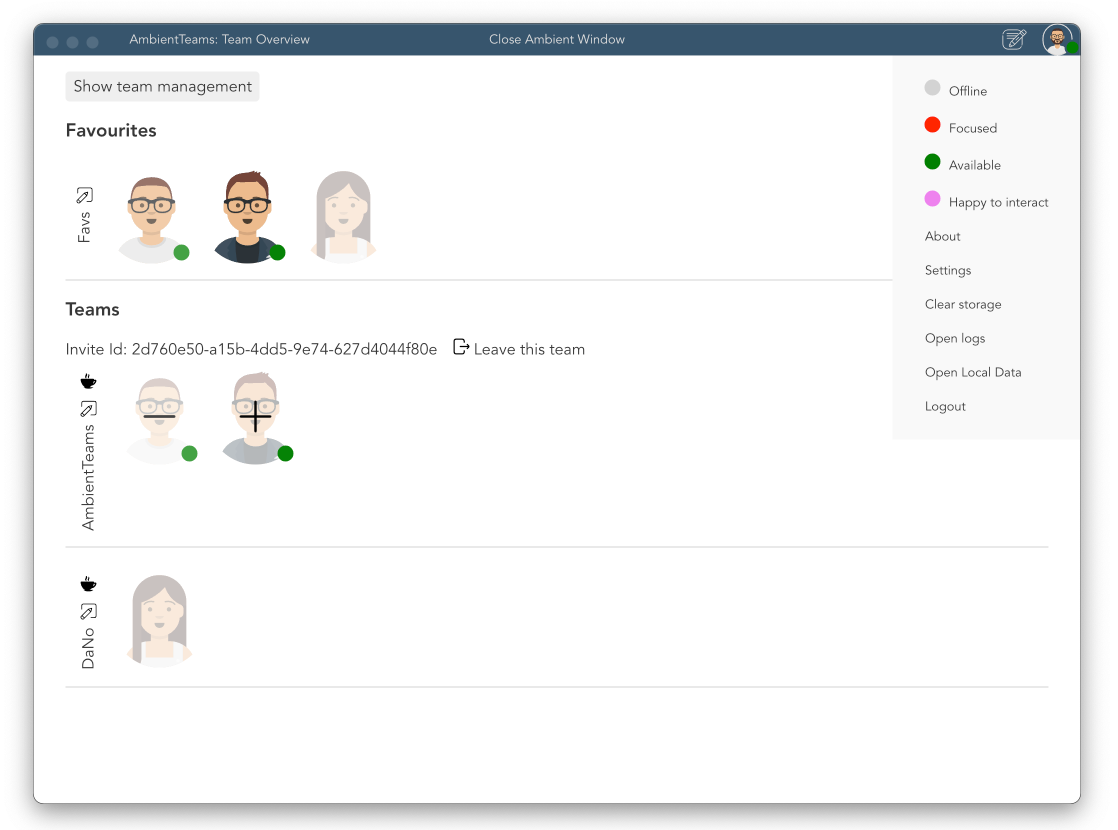
\includegraphics[width=.8\linewidth]{./images/AT_overview.png}
    \caption{Team Overview Window }
    \label{fig:at_overview}
\end{figure}

\subsection{Ambient, Glanceable Window}
\label{subsection:ambient_window}
The ambient window is always on top of other windows (see \autoref{fig:at_ambient_on_top}), which on the one hand, makes it easy to stay informed about moods and other statuses of your team members, but on the other hand, can also cause interruptions and distractions. We used a transparent borderless window to keep the ambient overlay as ambient and unobtrusive as possible. However, if the window is still distracting, it can be easily minimized or closed altogether using the menu that can be accessed by clicking the minimize icon (see \autoref{fig:at_hover}). By clicking on the three dots in the menu, which will reveal a small drop-down menu, the team overview window can be opened. Also, in this menu, the ambient window can be enlarged or reduced to fit different screen resolutions and personal preferences.

\begin{figure}[h]
    \centering
    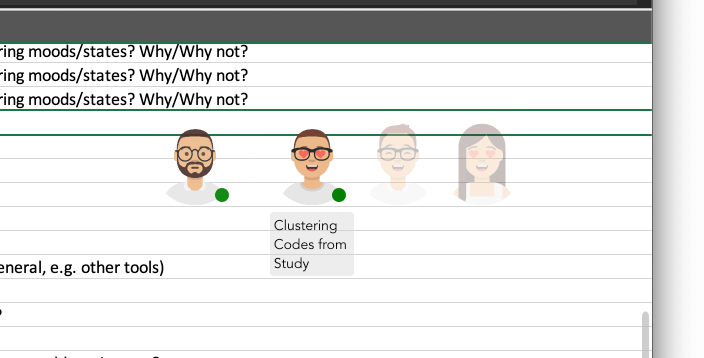
\includegraphics[width=.8\linewidth]{./images/AT_ambient_on_top.png}
    \caption{Always-on-Top Ambient Window While Working on Another Task}
    \label{fig:at_ambient_on_top}
\end{figure}

Further, certain elements are only visible when the user is hovering over this window (see \autoref{fig:hover_no_hover}). When hovering over the ambient window, the user can select the team they want to show and sees the names of the individual team members, as shown in \autoref{fig:at_hover}.

\begin{figure}[h]
    \centering
    \begin{subfigure}{.5\textwidth}
        \centering
        
\includegraphics[width=.8\linewidth]{./images/AT_no_hover.png}
        \caption{No Hover}
        \label{fig:at_no_hover}
    \end{subfigure}%
    \begin{subfigure}{.5\textwidth}
        \centering
        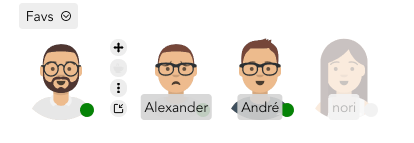
\includegraphics[width=.8\linewidth]{./images/AT_hover.png}
        \caption{Hover}
        \label{fig:at_hover}
    \end{subfigure}
    \caption{Ambient Window}
    \label{fig:hover_no_hover}
\end{figure}

\section{Availability Status}
For AmbientTeams we wanted to keep the number of interruptions to a minimum, which is why there is the \enquote{Focused} availability state (see \autoref{fig:call}) that exists in addition to the three others (\enquote{Available}, \enquote{Offline}, and \enquote{Happy to Interact}). Users in this focused state cannot be called. Further, they do not see any direct messages or incoming nudges until they leave the focused state. In addition, focused users cannot directly interact with other team members, avoiding potential self-distraction. The availability state \enquote{Happy to Interact} was included to address the lack of serendipity in remote work. When selected by at least two team members, an automatic matchmaker runs every minute and randomly pairs two people, who are then routed to a video call.

\section{Sharing Moods and Status Messages}
The user can open the sharing window from both the team overview and the ambient window, and the system tray menu. All of those actions will open the sharing window as shown in \autoref{fig:sharing_manual}, where on the left, a preview of the current avatar and the selection of available moods are listed. There are nine available moods, visualized using popular emoticons available through OpenMoji\footnote{\url{https://openmoji.org}}, an open-source emoji project. The first four of the available emoticons are more optimistic, the fifth is a neutral face, and the last four are emoticons representing rather negative emotional states. The selection of the emoticons started with six basic emotions: surprise, fear, disgust, anger, happiness, and sadness \autocite{an2017two}. This list was expanded over time to better suit the work environment by adding a neutral and tired emoticon and two more positive emotions (loving hearts and grinning) to make the selection more balanced. Due to limitations with the avatar API, we could not render \enquote{fear} well enough, which led us to remove it. On the right, the user can enter additional context in a simple, standard textbox. The contents of this textbox are, if available, pre-populated with the current status message for the currently selected team. Additionally, the text is highlighted when the window is created, facilitating overwriting the current status without using the mouse to select the text manually. The status messages' length is limited to 140 characters, motivated by the initial limit of Twitter \autocite{dullemond2013fixing}. Below the textbox, the user can find a button to share the status message with either all teams or a single team.

As a reminder for the user to share their moods and potential additional context with team members, the sharing window also appears automatically at pre-defined times. The location we chose for this popup is the lower right corner of the user's primary monitor to minimize the potential for distraction. Overall, the window has the same functionality but includes two additional buttons to defer the prompt for either 5 minutes or 1 hour (see \autoref{fig:sharing_auto}). The scheduled sharing window is displayed at three pre-defined times throughout the day, namely at 9:00, 13:00, and 16:00 local time. We chose those times because that is when most people are already or will still be working.

\begin{figure}[h]
    \centering
    \begin{subfigure}{.5\textwidth}
        \centering
        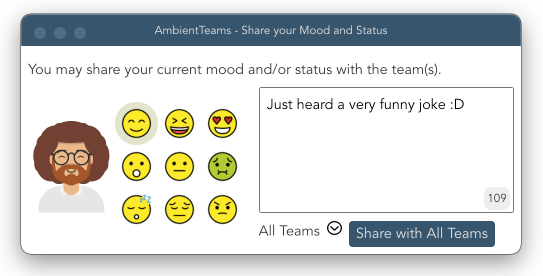
\includegraphics[width=.8\linewidth]{./images/sharing_manual.png}
        \caption{Manually Opened}
        \label{fig:sharing_manual}
    \end{subfigure}%
    \begin{subfigure}{.5\textwidth}
        \centering
        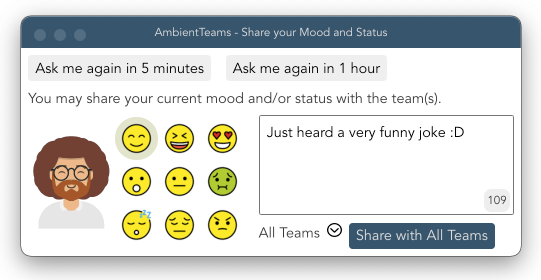
\includegraphics[width=.8\linewidth]{./images/sharing_auto.png}
        \caption{Scheduled}
        \label{fig:sharing_auto}
    \end{subfigure}
    \caption{Sharing Window}
\end{figure}

To ensure that the information shared within AmbientTeams is always up-to-date, a few measures have been taken. The first is purely visual: avatars are increasingly hidden the longer there has been no current activity. Such activities include status and mood sharing, direct messaging, and nudging. This automatic hiding should motivate users to interact with such hidden team members and easily spot updates from colleagues. Another measure we have taken to avoid showing users outdated content is automatically resetting status updates and moods at midnight.

Since the goal of AmbientTeams is to encourage informal communication, there is no chat history or other history built into the application. With this feature, we want to promote more casual and less formal communication and hope to avoid AmbientTeams becoming just another tool to keep track of.

\section{Ever-Running Breakroom}
As mentioned before, our goal was to create ever-running breakrooms as effortlessly as possible. \autoref{fig:breakroom_initiator} shows the state of the ambient window when the user has clicked on the coffee icon. After the user clicks on this coffee icon, the other team members will see an indication that there is a breakroom in progress (see \autoref{fig:breakroom_indicator}). However, to avoid unnecessarily creating a breakroom and potentially interrupting the initiating user, the breakroom is not created until another user clicks on the coffee icon.

\begin{figure}[h]
    \centering
    \begin{subfigure}{.5\textwidth}
        \centering
        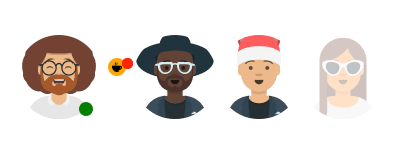
\includegraphics[width=.8\linewidth]{./images/breakroom_initiator.png}
        \caption{Initiating a Breakroom Creation}
        \label{fig:breakroom_initiator}
    \end{subfigure}%
    \begin{subfigure}{.5\textwidth}
        \centering
        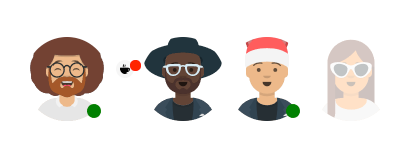
\includegraphics[width=.8\linewidth]{./images/breakroom_indicator.png}
        \caption{Joining a Breakroom }
        \label{fig:breakroom_indicator}
    \end{subfigure}
    \caption{Breakroom Creation}
\end{figure}

Once at least two team members have clicked the breakroom icon, a breakroom is created in the back-end with twilio\footnote{\url{https://www.twilio.com}}, and they are redirected to the breakroom view (see \autoref{fig:breakroom}). At any point, other team members can join and leave the breakroom, and it will remain active as long as at least one team member is present. We want to avoid users forgetting the time and staying too long in the breakroom. For this purpose, a 15-minute timer is started as soon as one enters the breakroom. When this timer reaches its end, the user automatically leaves the breakroom.

\begin{figure}[h]
    \centering
    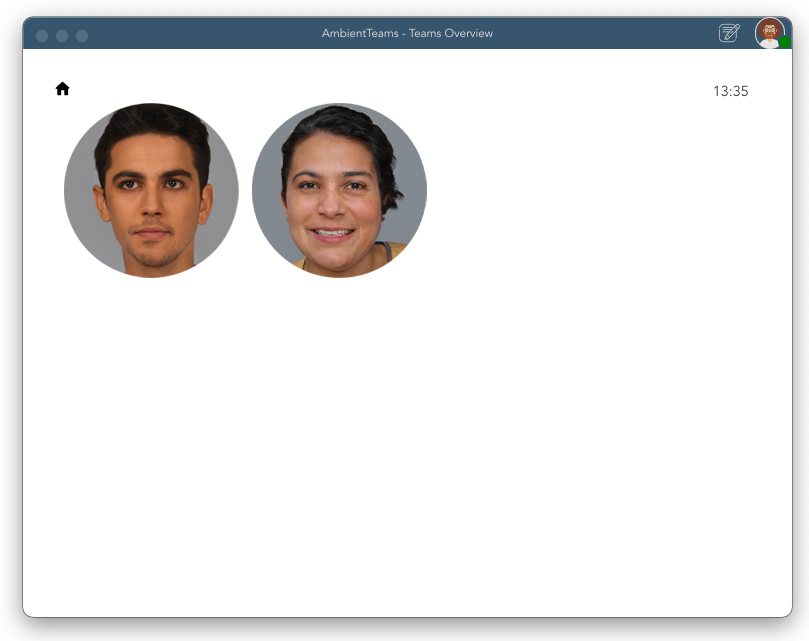
\includegraphics[width=.8\linewidth]{./images/breakroom.png}
    \caption{Ongoing Breakroom}
    \label{fig:breakroom}
\end{figure}

\section{Direct Interactions}
In addition to broadcasting moods and status messages, there is also the ability to interact directly with an individual team member. Hovering over individual team members brings up an overlay that offers three different interaction options, namely 1) direct messaging, 2) nudging, and 3) direct calling (see \autoref{fig:interactions}).

\begin{figure}[h]
    \centering
    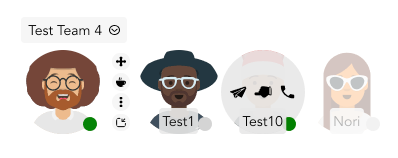
\includegraphics[width=.4\linewidth]{./images/interactions.png}
    \caption{Direct Interactions Overlay}
    \label{fig:interactions}
\end{figure}

Direct messaging is very similar to status message sharing but without mood sharing and team selection options. After clicking the message icon, the message window (\autoref{fig:messaging_window}) is displayed at the user's current mouse position to minimize the distance needed to interact with the window's contents. As in the status sharing window, there is a character limit of 140 characters.

\begin{figure}[h]
    \centering
    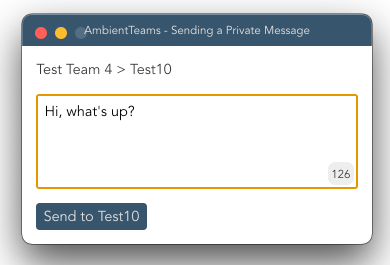
\includegraphics[width=.4\linewidth]{./images/messaging_window.png}
    \caption{Messaging Window}
    \label{fig:messaging_window}
\end{figure}

In \autoref{fig:interaction_results} all three interaction options are visualized. Direct messages (\autoref{fig:dm}) are distinguished from status messages by the message icon located to the left of the actual message. Nuding (\autoref{fig:nudging}) uses a hand icon pointing to the team member in question. For a video call (\autoref{fig:call}), the video stream overlays the team member's avatar, and the availability status of both participants is automatically set to \enquote{Focused}. Users can hover over their avatar if they want to mute or pause the video stream. To end a call, you need to hover over the corresponding team member and click the hang-up icon.

\begin{figure}[h]
    \centering
    \begin{subfigure}{.3\textwidth}
        \centering
        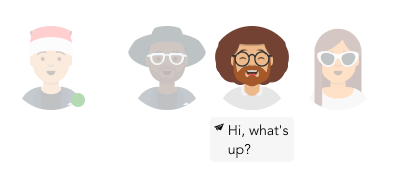
\includegraphics[width=.9\linewidth]{./images/DM.png}
        \caption{Direct Message}
        \label{fig:dm}
    \end{subfigure}%
    \begin{subfigure}{.3\textwidth}
        \centering
        
\includegraphics[width=.9\linewidth]{./images/nudging.png}
        \caption{Nudging}
        \label{fig:nudging}
    \end{subfigure}
    \begin{subfigure}{.3\textwidth}
        \centering
        
\includegraphics[width=.9\linewidth]{./images/call.png}
        \caption{Ongoing Video Call }
        \label{fig:call}
    \end{subfigure}
    \caption{Direct Interactions}
    \label{fig:interaction_results}
\end{figure}
\chapter{Preliminary Evaluation}
\label{chapter:preliminary_evaluation}
To evaluate the above mentioned research questions, a preliminary evaluation is conducted. Optimizing and improving our approach with the help of feedback from the participants is the primary goal of this master thesis. Further, we want to learn which status and moods knowledge workers share with their closest team members, what they learn from their team-mates' sharing and the overall impact on their perception of workplace isolation.

TODO: Quickly describe \autoref{fig:study_timeline} in words before jumping into more details in the following sections.

\begin{figure}[h]
    \centering
    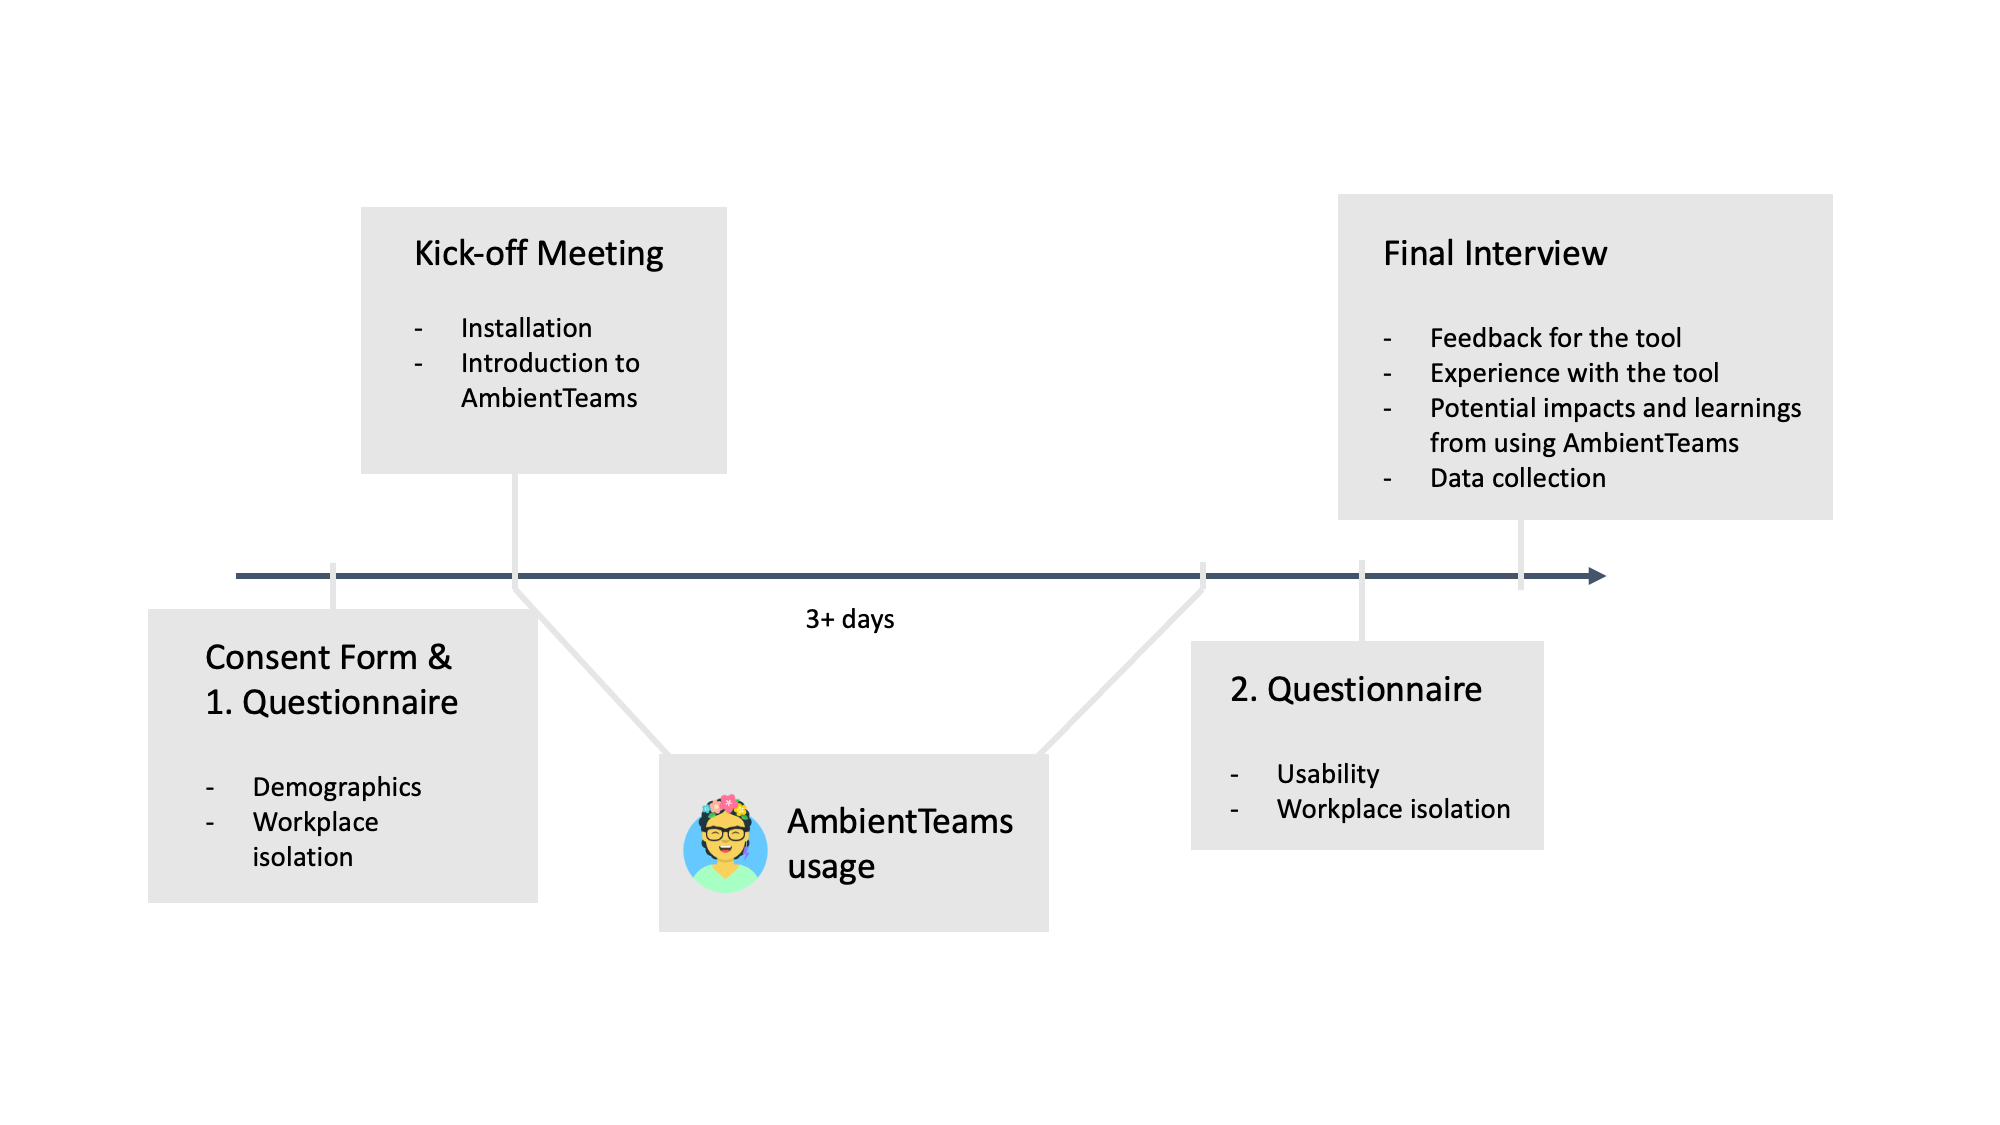
\includegraphics[width=.8\linewidth]{./images/Study_Timeline.png}
    \caption{Study timeline}
    \label{fig:study_timeline}
\end{figure}

\section{Participants Recruitment}
\label{section:recruitment}
As a first step, an interested team had to be recruited. To that end, the researchers' personal network will be used. To that purpose, the study description is forwarded to the contacts, and once an interested team has been identified, it is checked whether it fulfills the participation criteria and if the prospective participants are (technically) allowed to install AmbientTeams on their computer. If this is not the case, the company's consent and approval to install AmbientTeams is first obtained. To provide the company with as much information as possible about the study and the privacy/confidentiality of the data collected during the study, the consent form and a study description will be given to the company for review. After gaining the company's approval, the individual interested team members are approached by presenting the study, discussing the steps and goals of the study, and emphasizing that participation is entirely voluntary.

The requirements for teams participating were as follows:

\begin{enumerate}
    \item At least three team members
    \item Three or more common working days a week
    \item Spending the majority of their workday on the computer
    \item Having all the required rights to install AmbientTeams on their work computer
    \item Willingness to use AmbientTeams during at least three full days of work (approximately 0800 - 1700)
    \item Using macOS or Microsoft Windows
    \item An active internet connection
\end{enumerate}

\section{Participants}
With our recruitment, we were able to find an interested team. TODO: Describe team

\section{Initial meeting}
\label{section:initial_meeting}
Installation

\section{Prestudy Questionnaire}
\label{section:prestudy_questionnaire}
The questions are taken from ....

\section{Evaluation Phase}
\label{section:evaluation}
How long? \\
During the study notes from notion

\section{Poststudy Questionnaire}
\label{section:poststudy_questionnaire}
The questions are taken from ....

\section{Interview}
\label{section:interview}
Interview questions and their relevance for the research questions
\chapter{Results and Discussion}
\label{chapter:results_and_discussion}

This chapter presents and discusses the results that we found through analyzing the collected data (see \autoref{table:data}), results from the semi-structured interviews, and findings from the two questionnaires.

\section{Usability}
\label{section:usability}
%  more info on usability score: https://measuringu.com/sus/
% A SUS score above 68 would be considered above average, and anything below 68 is below average.
% # A SUS score of 74 has higher perceived usability than 70\% of all products tested. It can be interpreted as a grade of a B-.

The results from the usability questionnaire which the participants answered at the end of the study are shown in \autoref{fig:usability_questionnaire}. For the questions with even numbers, e.g., Q2, Q4, etc., negative answers are desirable, whereas, in questions with uneven numbers, e.g., Q1, Q3, etc., positive, blue responses are ideal. Generally, the result looks very promising. There are, however, some answers worth discussing. The \enquote{disagree} answer from Q1 came from P586. P586 also disagreed that the various functions of the application were well-integrated (Q5). The reasons for these answers could be found in the interview, where the following statement was made.

\begin{displayquote}
    Uhm, as a separate tool, I would not use it. Integrated into another communication tool, I might use it, yes. -P586
\end{displayquote}

The \enquote{agree} response in questions Q4 and Q10 came from P163, indicating that the number of featured in AmbientTeams is quite demanding to understand simply during the initial meeting. Nevertheless, this participant did not mention any usability issues in the interview nor through direct feedback, leading us to believe that it was straightforward to use after the initial challenge of understanding the application.

\begin{figure}[h]
    \centering
    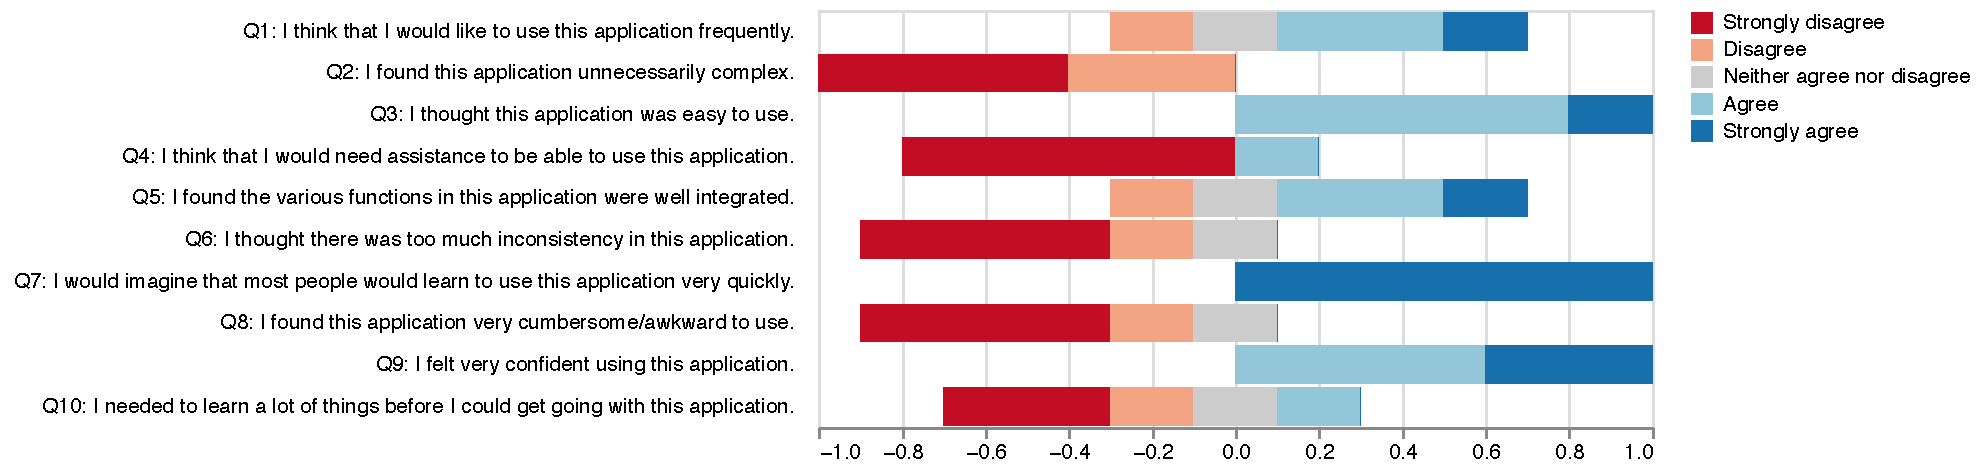
\includegraphics[width=\linewidth]{plots/usability_likert.pdf}
    \caption{Usability questionnaire results}
    \label{fig:usability_questionnaire}
\end{figure}

The individual participants' answers were then converted into the SUS score for each question according to \textcite{sauroSUS} to get a comparable score. The resulting average SUS score was 81.1 across all five participants (see \autoref{table:sus}). According to \textcite{sauroSUS}, one would need to score above 80.3 to be in the top 10\% of the 500 studies using the SUS. 80.3 is also the point where users are more likely to be recommending the product to a friend \autocite{sauroSUS}, making us believe that AmbientTeams was easy and intuitive to use.

\begin{table}[h]
    \centering
    \begin{tabular}{|l | l|}
        \hline
        Participant & SUS score \\
        \hline
        P038        & 82.5      \\
        % \hline
        P163        & 80.0      \\
        % \hline
        P586        & 70.0      \\
        % \hline
        P751        & 82.5      \\
        % \hline
        P904        & 90.5      \\
        \hline
        Average     & 81.1      \\
        \hline
    \end{tabular}
    \caption{Usability questionnaire results and resulting SUS score}
    \label{table:sus}
\end{table}

\section{Tool Usage and Workflows (RQ4)}
\label{section:tool_usage_and_workflows}

A detailed timeline view of the participants and their selected availability state (\enquote{Available}, \enquote{Focused}, or \enquote{Happy to interact}) throughout the study is visualized in \autoref{fig:non_offline}. Those three states combined are looked at as the time when the application was running (potentially in the background). This is because the user is automatically set to an offline state if the connection to the server is lost. Upon successful connection to the server, the user's availability state is also automatically set to \enquote{Available}. It is worth mentioning that this metric could be slightly erroneous if participants manually set their availability status to \enquote{Offline}. This would, however, only underestimate the time spent online in \autoref{fig:non_offline}, making our results as conservative as possible. All in all, the average time spent in a non-offline state, and thus AmbientTeams was running (potentially only in the background), was 7.13 hours per day (std. 3.57), with a minimum of 0 and a maximum of 12.7 hours. Except for the inactivity on the weekend, only some participants did not use AmbientTeams some days. To be precise, only 5 out of a total of 30 workdays showed no or very short running time. The fact that P038 could not participate in the initial meeting with the rest of the group explains the lack of usage on the first day of the study. In general, because the kick-off meeting took place in the early afternoon, the relatively short running time on the first day was to be expected. The remaining days with very little only time most likely indicate non-working days for those participants because had they worked on those days, AmbientTeams would have automatically started as soon as they had started up their computer.

\begin{figure}[h]
    \centering
    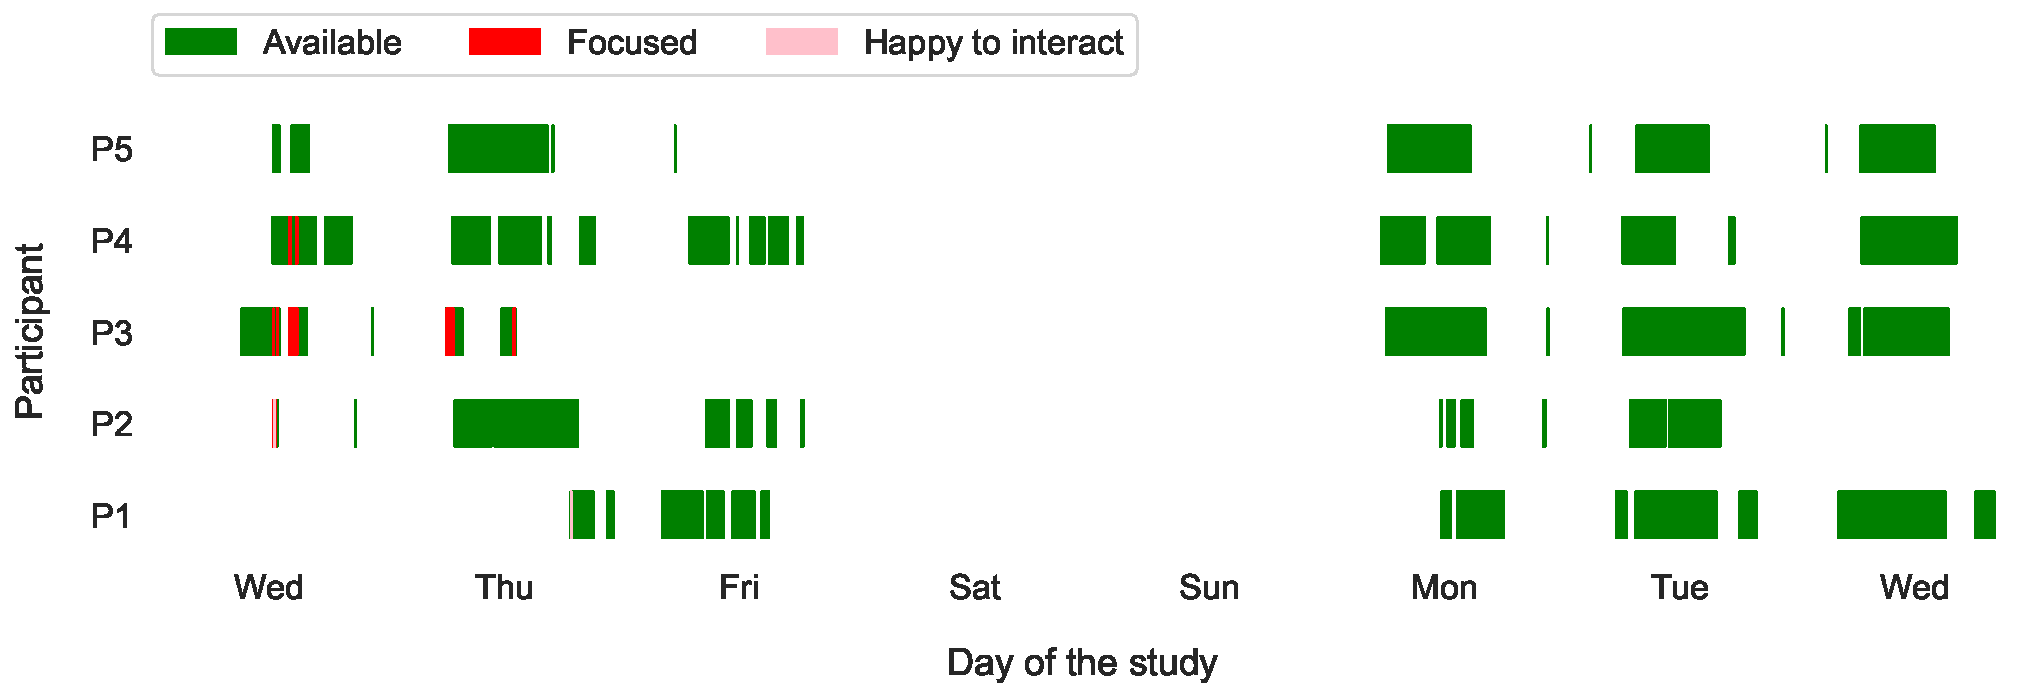
\includegraphics[width=\linewidth]{plots/non_offline.pdf}
    \caption{Time spent in the different availability states}
    \label{fig:non_offline}
\end{figure}

The results show that the participants did not often change their availability states and thus mainly relied on the automatic availability status setting of AmbientTeams. The \enquote{Focused} state was selected a couple of times in the first two days of the study, yet this behavior did not continue throughout the study.

\subsection{Challenges and Novelty of the Ambient Window}
\autoref{fig:opened_vs_focused} illustrates that both the ambient window and the team overview window were almost exclusively opened when those windows were in focus. In other words, both of those windows were opened, interaction took place, and then they were closed or minimized again, making them disappear from the user's monitor. This is the result we expected to happen in the case of the team overview. In contrast to our beliefs, however, the ambient window was used very similarly. As a result, the ambient window only very rarely was kept open as a glanceable, always-on-top team view when working on other tasks.

\begin{figure}[h]
    \centering
    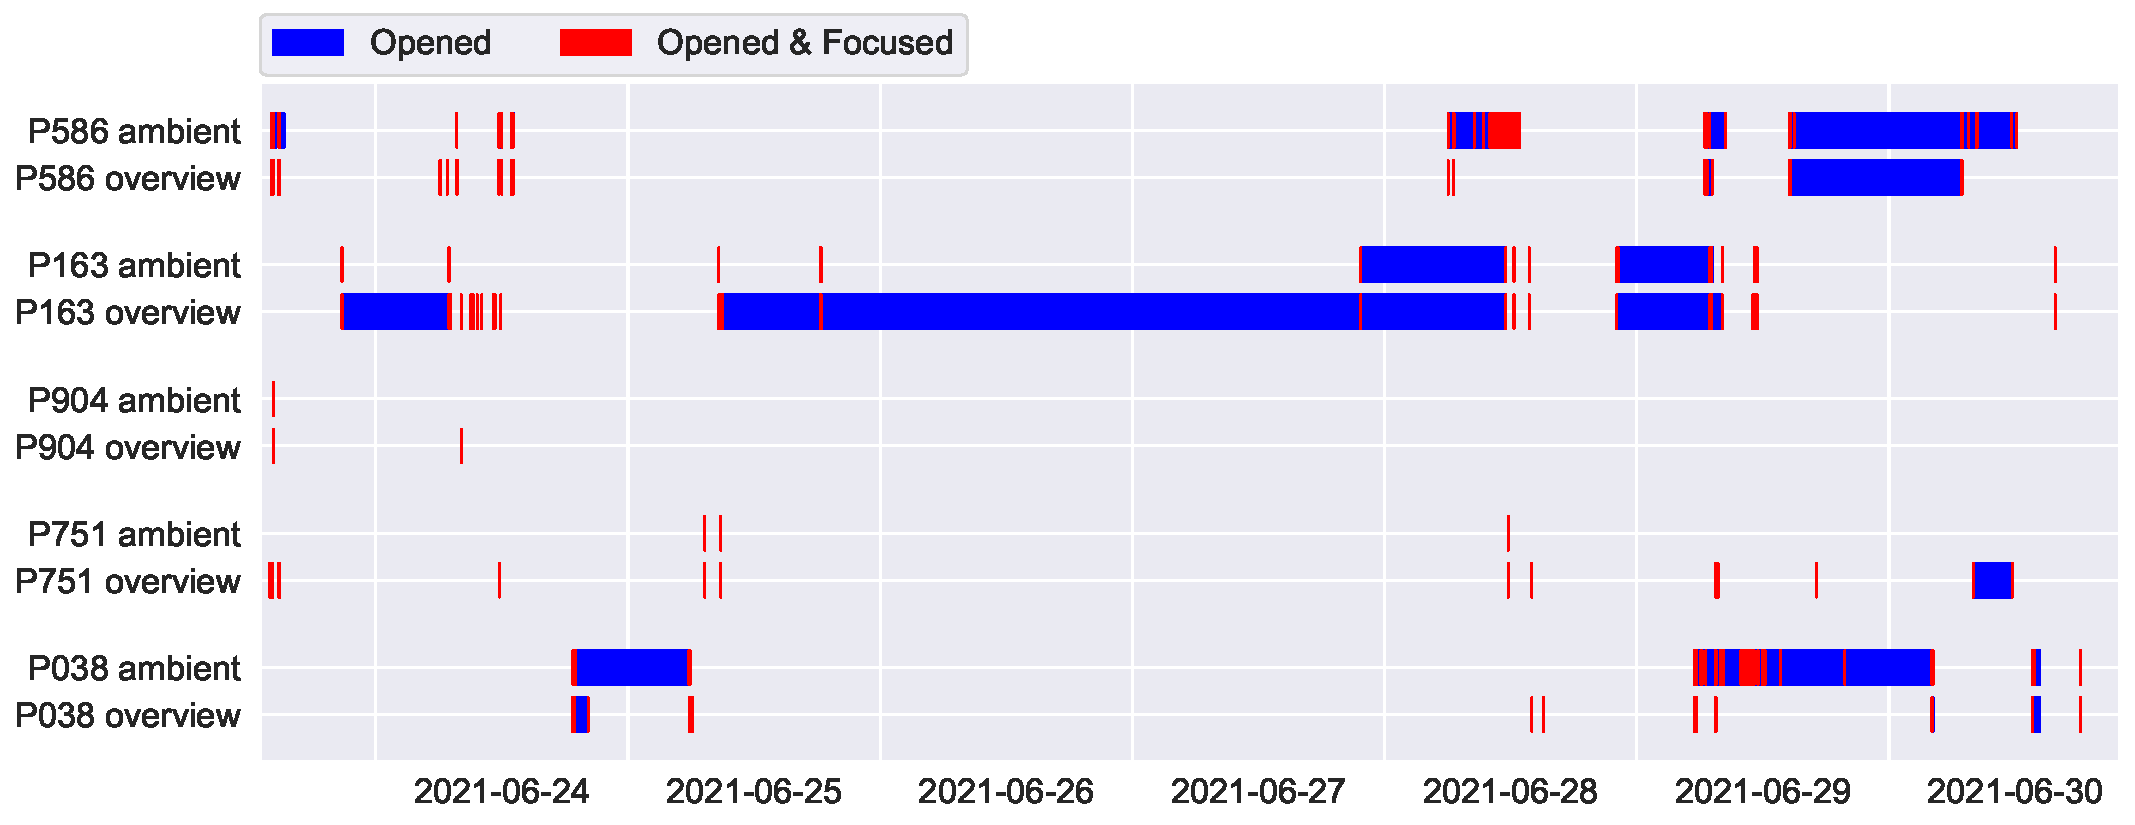
\includegraphics[width=\linewidth]{plots/open_vs_focus.pdf}
    \caption{Time AmbientTeams was opened vs. opened and focused}
    \label{fig:opened_vs_focused}
\end{figure}

The interviews gave us some more insights into possible answers for why the ambient window was not kept open while working on other tasks.

\begin{displayquote}
    I tried it in the corner of the monitor, then it did not work, but in the corner of the window did not really work because there you have to click to close other windows. Then I put it somewhere in the middle, but then I needed to put some buttons there, so sometimes I got annoyed and then closed it. -P038
\end{displayquote}

We hypothesize that this particular user most likely was using a single monitor setup and had a hard time finding a suitable position for the ambient window. P586 mentioned that the ambient window was too small and thus too difficult to properly move around, indicating that this participant might have missed this part of the demonstration during the kick-off meeting. In addition to the annoyance of the ambient window experienced by P038 and P586, P163 mentioned that manually closing an application that automatically starts up is something that happens almost automatically to them because of established habbits. The hassle and difficulties of positioning the ambient window are a rather crucial issue that potentially requires further development; the case described by P163 could be solved by not allowing to close the ambient window during a future study.

To make the ambient window fit better into their workflow, P038 suggested that it should ideally not stay on top of other windows and instead just come to the foreground again once a team member has shared something new. P586 similarly suggested that the ambient window ideally should fade out when not being used.

Despite the criticism around the ambient window, it was still used by all the participants except for P904 and seen as one of the best aspects of AmbientTeams by P751:

\begin{displayquote}
    I liked that the ambient window feels very dynamic and refreshing compared to other tools. -P751
\end{displayquote}

Despite this positive statement, this participant used the team overview window more, which is surprising because all the participants were only part of one team during the study, eliminating the potential advantage of the team overview window, in our opinion.

\section{A Need for Status and Mood Sharing (RQ1)}
From the interviews, we could identify two reasons why there is a need for mood sharing at the workplace: the lack of 1) awareness and 2) social interactions in remote work environments. This finding further confirms our motivation to create AmbientTeams in the first place.

\medskip\noindent\textbf{Lack of Awareness} \\
P163 explained that there is a lack of awareness of the \textit{real} mood when working remotely. Even though you might see them during video conferences, it makes the impression that feelings expressed through such calls might not be real.

\begin{displayquote}
    I think it's a good idea, especially now if you work either hybrid or completely remote, I think then it is quite difficult to see the mood of your team colleagues, because now in most video conferences you make a happy face into the camera, so it is also difficult to see your mood how your mood really is right now. -P163
\end{displayquote}

To highlight this point more, four out of five participants mentioned in the pre-study questionnaire that they are not or only partially aware of their co-workers' moods. This is because of missing cues resulting from working from home, according to P586.

\begin{displayquote}
    I like to ask people how they feel but being in a room with your colleagues gives you more information about how someone is actually feeling. -P586
\end{displayquote}

Those two statements both talk about the concept of honesty in regards to expressing feelings, a topic that was, unexpectedly, talked a lot about during the interviews and will therefore be covered in more detail in \autoref{section:negative_moods_and_honesty}.

But why is mood awareness important? Being aware of your co-worker's feelings is essential for personal relationships, something important, says P751.

\begin{displayquote}
    Yes, it [feeling of co-workers] is important to me because if you think about how much time you spend with your co-workers, it is very important that you have good personal relationships with those people. Even when it's not clear how much longer you will be working together with those people. -P751
\end{displayquote}

In addition, certain conclusions about the current workload of employees can also be drawn through the exchange of moods and states, facilitating task assignment.

\begin{displayquote}
    Sometimes I then [at a previous company] got the feedback that they already finished with work or that they have no more tasks left. With something like AmbientTeams they could set like a bored state, and I would have been able to give them a new task. -P163
\end{displayquote}

\medskip\noindent\textbf{Lack of social contact / task-focus} \\
One participant (P032) talked about how working remotely often is very task-centric, which leads to forgetting about the \enquote{social aspects of an enterprise}. P586 mentioned that when working remotely, communication often is limited to be very business-focused, and conversations are therefore usually only started for business reasons.

\begin{displayquote}
    I think during corona, you don't really have that breakroom time, so if you call somebody, it's mostly about business and not about private stuff. So, I think it's very difficult to get into a deeper connection with people you don't see that often. -P586
\end{displayquote}

To conclude, there appears to be a need for some mood and status awareness-providing approach. The following sections look into how our approach, AmbientTeams, performed at tackling the challenges mentioned above.

\section{Moods Were Shared the Most (RQ2)}
Moods were the most actively shared states, with a total of 31 moods being shared. In contrast, only eight status messages were shared, three of which were in reaction to Switzerland's soccer game during that time. Generally speaking, none of the status messages contained any work-related information.

\begin{figure}[h]
    \centering
    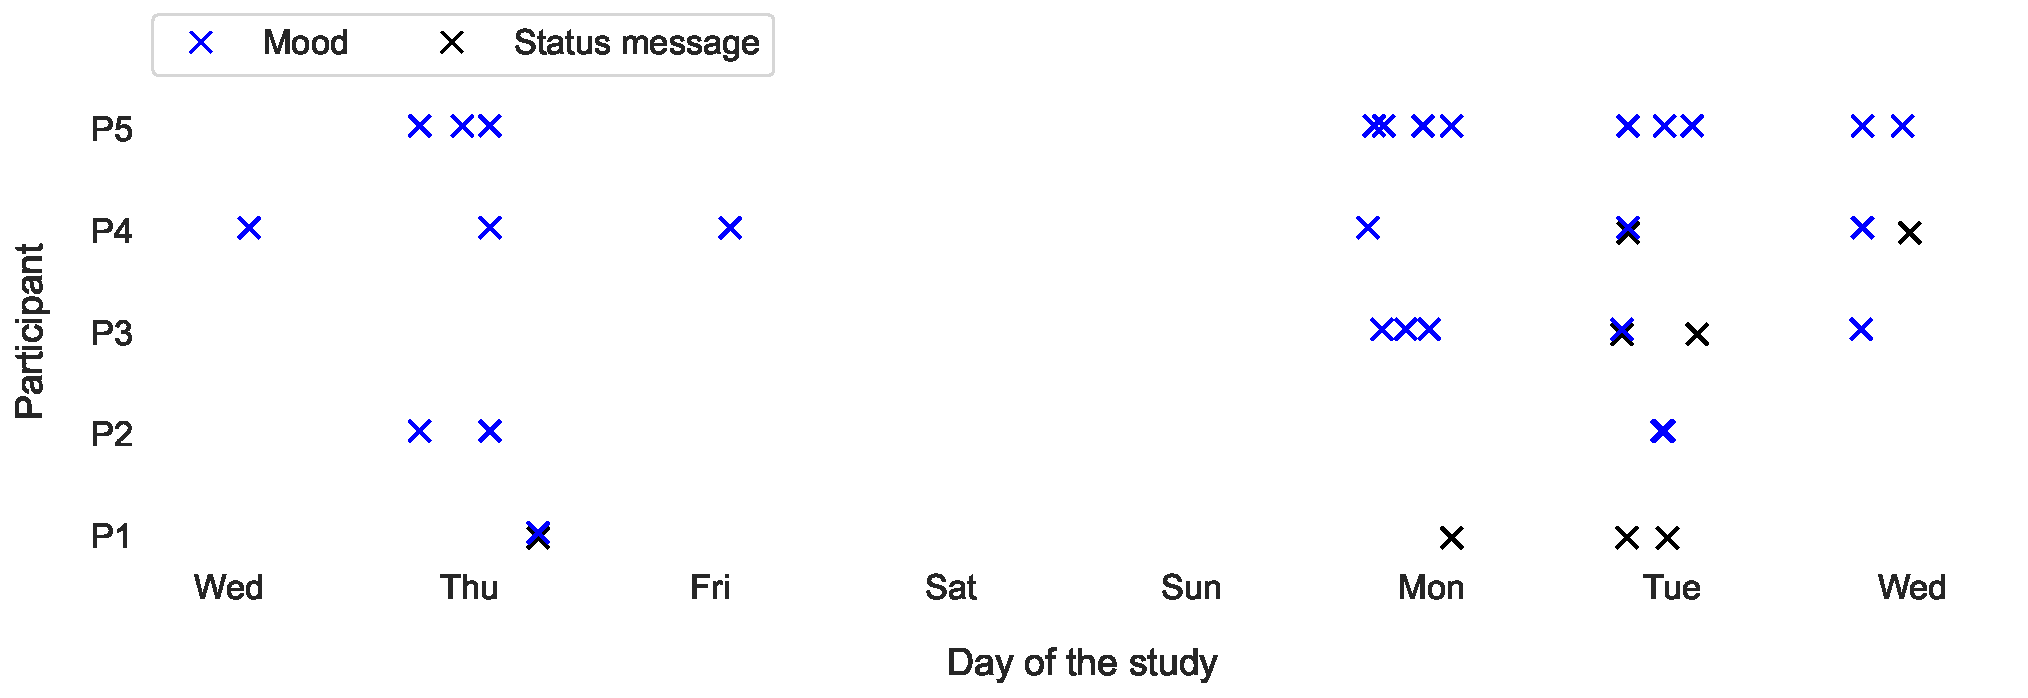
\includegraphics[width=\linewidth]{plots/moods_status_messages.pdf}
    \caption{Moods and status messages shared}
    \label{fig:moods_status_messages}
\end{figure}

Looking at \autoref{fig:moods_status_messages} shows that in only three cases, moods and status messages were shared simultaneously. According to the interviews, a primary reason for sharing moods was the automatically scheduled popup, which helped to remind the participants to share something. The data confirm this finding; 25 of the 32 shared moods were shared through the scheduled popup window. However, the participants usually just shared the mood through an emoticon and did not attach a text message. From P163, we learned that a potential reason could be that it was simply a lot quicker only to share the mood via emoticon, requiring only one click. P904 also mentioned that he/she did not see a reason to provide any more information to their mood (which was \enquote{tired} ten out of 12 times). TODO: Check if all three were negative.

While the scheduled popup helped remind the participants about sharing something, the motivation to share moods seemed to be that they knew the importance of communicating moods or interacting with co-workers (Pxxx). P586 also described how knowing that co-workers share the same feeling increases the likelihood of sharing this feeling yourself.

\begin{displayquote}
    And just this thing that I said before, if you have something that you are very happy about, you think that other people also share, then you are more motivated to share it as well. -P586
\end{displayquote}

% \begin{displayquote}
%     If we were not in a test phase, maybe I would not share that much if I saw that the others are also not really sharing anything. \\
%     -P586
% \end{displayquote}

Considering the relatively short time AmbientTeams was actively used, it is not surprising that many of its features were not used. More concretely, the features aimed at spontaneous interactions such as the breakroom and the random pairing for a video call were not used at all. While there have been two attempts of creating a breakroom, one on the second day of the study and one on the second to last day, none of them were successfully created because no other team member joined. P586 gave a possible explanation for why the spontaneous video chat features were not used during the interview.

\begin{displayquote}
    But also maybe I have to mention that two or three weeks ago we started with virtual break rooms on Friday afternoons to try to keep up with people from work, especially for new people, because we don't really get the chance to get to know each other in home office. -P586
\end{displayquote}

Consequently, it is possible that it is sufficient for the participating teams to meet once a week in their own virtual break room. Regardless of the use of the break room integrated into AmbientTeams, this indicates that the concept of such a break room is generally perceived as important. Similar to the breakroom, the directed video calls and the nudging functionality were only used during the initial kick-off meeting for testing purposes. While this shows that it was clear to the team how to use those features, they don't seem to have felt the need for those.

Things look a bit different when analyzing the direct messages that were sent through AmbientTeams. In total, there were six direct messages sent through AmbientTeams, coming from three different participants. One of those direct messages was a response to a missed call, and the other five were of either of type greeting or along the lines of \enquote{what are you doing?}. P032 gives an indication to why the team did not use the above-described functionalities:

\begin{displayquote}
    Because now it's a bit, you know I can write to somebody in Microsoft Teams or AmbientTeams, and I would normally pick MS Teams because we use it, and you also have a message history which you don't have in AmbientTeams. -P032
\end{displayquote}

Essentially, P032 explains that AmbientTeams has to differentiate itself from MS Teams, and it is doing so with the \textit{Twitter approach} of broadcasting moods and messages, but not so much with other communication functionalities.

\section{Negative Moods and Honesty (RQ2)}
\label{section:negative_moods_and_honesty}

When looking at \autoref{fig:moods_distribution}, it becomes apparent that, except for P904, who pretty much constantly was \enquote{Tired}, the most frequently shared moods were positive (especially \enquote{Happy}).

\begin{figure}[h]
    \centering
    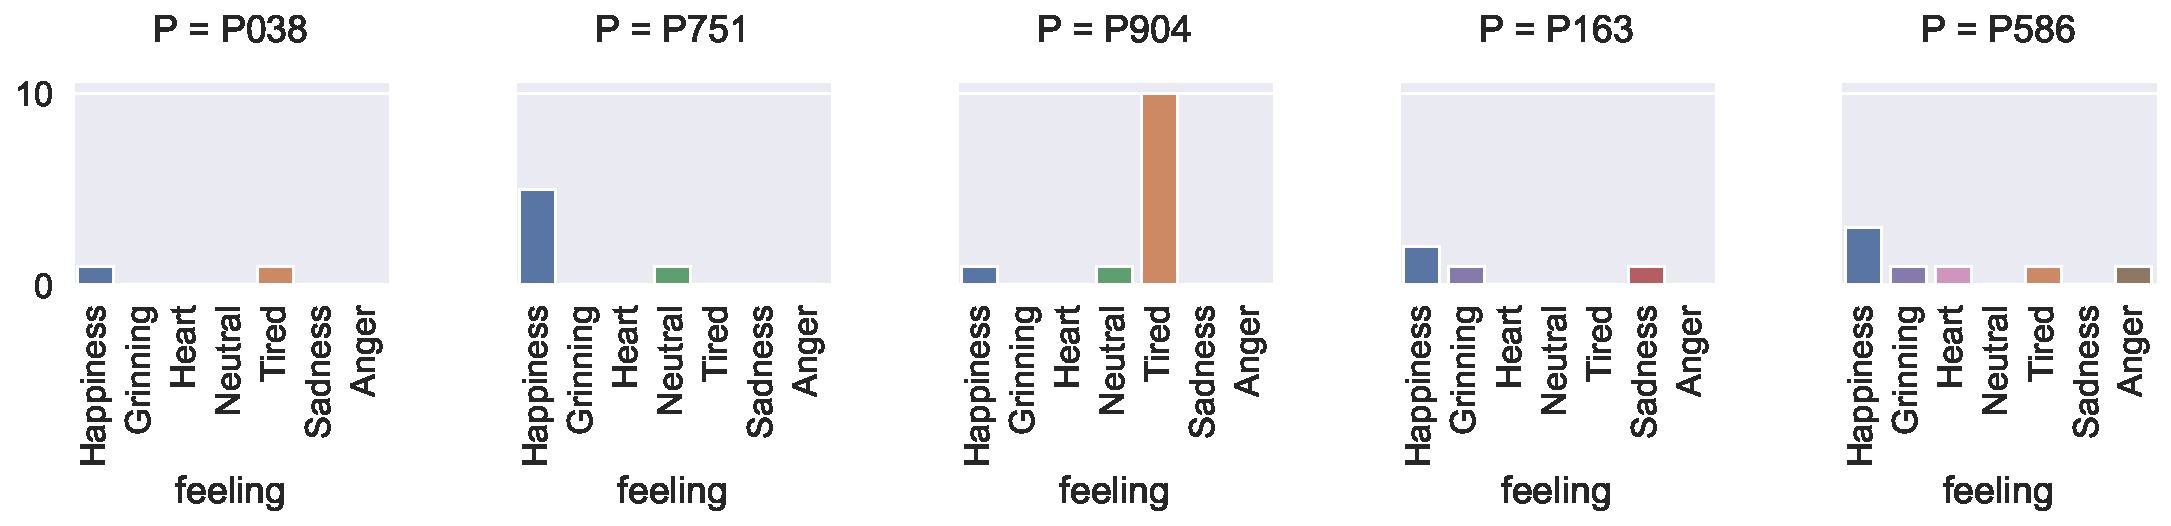
\includegraphics[width=\linewidth]{plots/moods_distribution.pdf}
    \caption{Distribution of shared moods }
    \label{fig:moods_distribution}
\end{figure}

Therefore, this finding raised the question, whether this was the real distribution of moods during the study or whether there could be a positive bias in moods when sharing. While P038 does not see a problem with sharing negative moods, because it's \enquote{normal, we are not in a happy boat where everyone is happy all the time}, others (P163, P586, P163) would be more hesitant to share such moods. Reasons for not sharing negative moods include 1) \textit{not wanting to give further explanations}, either for private reasons or not wanting to be distracted (P163), 2) \textit{being fairly new to the company} (P751), 3) \textit{not wanting to share them with the entire team} (P586), or 4) because \textit{nobody wants to talk about negative feelings at work} (P586).

% \begin{displayquote}
%     Yes, I think then it would be harder to share an angry mood. And if you are mad for private reasons, you maybe don't want to explain more. \\
%     -P163
% \end{displayquote}

% \begin{displayquote}
%     I would not share those things, like when I am tired or angry. \\
%     -P586
% \end{displayquote}

P751 further differentiates between the severeness of the experienced moods:

\begin{displayquote}
    I don't think I would share regular negative moods when having a bad day, for instance, being this new to a company. If something really severe were to happen, however, let's say something personal or family-related, I would share such moods to inform other people. -P751
\end{displayquote}


% \begin{displayquote}
%     But I always said that at this time that I had a good mood, this time this was honest, but I am not sure whether I would also share it if one day I had a bad mood. I am not sure if I then would be that honest to share it then directly online. \\
%     -P163
% \end{displayquote}

% -> Potentially undesired interruptions

% \begin{displayquote}
%     First reason is if I make, for example, an angry or sad mood, then everyone would text me, and I think I will maybe lose my focus because they would ask me why I was feeling in this way etc. And I think the second reason is that in the online world it is a lot easier to hide bad feelings, and you try to present yourself in the best way. \\
%     -P163
% \end{displayquote}

% \begin{displayquote}
%     It's easier to share positive feelings within a working environment compared to negative feelings because nobody wants to talk about negative feelings. \\
%     -P586
% \end{displayquote}

% While P586 also claims that talking about feelings is very important, sharing such personal information is not something that he/she likes to do.

% \begin{displayquote}
%     I mean of course it is very important that you talk about these kinds of things [feelings], but you don't want to share it with the whole team. \\
%     -P586
% \end{displayquote}

\section{Increased Awareness of Who Is Around and How They Feel (RQ3.1)}
The first effect of AmbientTeams was that participants learned who is around (P032, P586) and how they were feeling (P032, P751). P904 further noticed a key difference compared to their previous way of exchanging moods and feelings, which was usually done over text in the morning:

% \begin{displayquote}
%     Also, sometimes for just checking who is online and who is grayed out. -P586
% \end{displayquote}

\begin{displayquote}[][]
    [...] I wouldn't have known how you were doing during the day without AmbientTeams. [...] And, I think that's when you get additional information about how you're doing during the day. -P904
\end{displayquote}

This increased awareness had more implications, namely the possibility of getting to know each other better and bringing back a more natural way of communicating when working remotely. We will elaborate on both in the next sections.

\section{Getting to Know Each Other Better (RQ3)}
AmbientTeams led to one person (P751) in particular finding out that a colleague was very funny, which was unknown before the study.

\begin{displayquote}
    Yes, actually about one particular person in the team. I did not know that this person was so funny before using AmbientTeams. The fact that I got to know one person a lot better during this one week and also having non-work-related talks now already exceeds my expectations for the study, to be honest. -P751
\end{displayquote}

It is no surprise that P751 was pretty new to the company and thus did not have the chance to get to know all the team members too well. Due to this, this participant liked the fact that \enquote{this feature [mood sharing] allows to discover more about your colleagues, and it sheds light into a part that we tend to keep only for ourselves}, in particular seeing \enquote{moods and states of team members with whom I might not be currently working together too closely}. While the other participants did not learn something new about other people, P586 mentioned that using AmbientTeams confirmed the previous assumption \enquote{one team member is really just always very positive and too nice}, showing that there were in total two team members who took away a promising finding from the one week study.

We thus conclude that AmbientTeams has the potential to get to know individual team members better, especially for new team members, and learn more about team members with who you might not be in constant exchange.

% \begin{displayquote}
%     Not really, to be honest. I just had the confirmation that one team member is really just always very positive and too nice. -P586
% \end{displayquote}

\section{Bringing Back \enquote{Natural} Communication}
This section demonstrates the capabilities of AmbientTeams to bring back the more \enquote{natural} communication known from traditional office work to a remote environment. Such communication is enabled by providing \enquote{a lot more opportunities to approach another} (P904). P038 explains that by sharing moods and status with the entire team, everyone can see it, similar to when the entire team is in the office, and as a consequence, can react to what's been shared:

\begin{displayquote}[][]
    [...], but I actually found it if you share it with the whole team. Because sometimes people then come back to you that you don't expect. So I mean, sometimes you don't have a good mood and people see it and want to cheer you up. So this substitutes a bit that part of the office life. -P038
\end{displayquote}

Another reason for how AmbientTeams can trigger communication includes \textit{seeing when someone comes online} (P032), which resulted in contacting this person. We see this as the equivalent of going into the office and being reminded of something that needs to be done simply by seeing your co-workers. Also, the fact that the majority of the participants would not necessarily share negative moods, P163 mentioned that he/she would still offer help in cases of an angry or stressed mood, another possible communication trigger.

Despite P163 pointing out that AmbientTeams itself makes it easy to start a conversation by \enquote{only having to click on the avatar of [...] to start a conversation}, this was not observable in the collected data. However, what we could observe, and this was also brought up during the interviews by P751 and P032, was that AmbientTeams acted as a trigger for external communication (e.g., Microsoft Teams, Zoom.us, etc.). To that end, we analyzed the active window titles of the participants during the study to see whether there is a higher chance of visiting external communication apps after leaving AmbientTeams.

TODO: Charts/Numbers about external triggers.

% \begin{displayquote}
%     I had more non-work-related communication, however, outside of AmbientTeams in our existing tool. -P751
% \end{displayquote}

% \begin{displayquote}
%     So, for example, I saw that somebody pushed \enquote{good morning}, then I thought \enquote{ahh okay I need to speak to this person about some topic}, so I called this person on MS Teams. -P038
% \end{displayquote}

% Reason: Lower barrier

% \begin{displayquote}
%     Yes, definitely. It provides a lot more opportunities to approach another. -P904
% \end{displayquote}

% \begin{displayquote}
%     Because if you only have to click on the avatar of Zsuzi or Adelina to start a conversation. -P163
% \end{displayquote}

% Reason: Help offering

% \begin{displayquote}
%     I think in that study not. But if somebody would have set an angry or stressed mood I would have helped him/her, if my current knowledge allowed it. -P163
% \end{displayquote}

\section{Mood Awareness via Self-Reflection (RQ3.2)}

\begin{displayquote}
    But I think it impacted myself because you're always prompted to think about your own mood. -P751
\end{displayquote}

In the previous sections, we presented results depicting the effect of AmbientTeams on other team members. However, we also found impacts on the person sharing moods themselves. More concretely, the self-reflection side of AmbientTeams was talked about by three people (P751, P904, and P586). P904 realized how their moods changed: \enquote{then maybe a few hours later you realized, I'm actually not tired or not so neutral, but rather happy}. We argue that mood awareness via self-reflection is something that could have many more applications and benefits. During the interview, one participant even gave a concrete example of how reflecting on moods could help find potentially hidden areas of interest.

\begin{displayquote}
    If I had something that could then show me afterward that for example, every time I do something for IT I am very happy, then I can maybe try to seek more tasks in IT and find my potential in IT and my life itself to make any further education for instance. -P586
\end{displayquote}

\section{Workplace Isolation (RQ3.4)}
\label{section:workplace_isolation}

The sections above can already hint at the capability of AmbientTeams to reduce the feeling of workplace isolation within knowledge work teams. This highly qualitative data was complemented with our approach to measure workplace isolation quantitatively; a questionnaire was asked before and after the study period. Before looking into the results of the questionnaire in \autoref{fig:workplace_isolation}, a mistake from our side made us adjust the scale. The original workplace isolation questionnaire provides for a 7-point Likert-Scale. Unfortunately, our post-study questionnaire included a flaw where its answer range only was a 5-point Likert-Scale. To make the two somewhat comparable, the answers from the pre-study questionnaire for \enquote{somewhat disagree} and \enquote{disagree} were combined into \enquote{disagree}, and similarly the answers for \enquote{somewhat agree} and \enquote{agree} were combined into \enquote{agree}.

\begin{figure}[h]
    \centering
    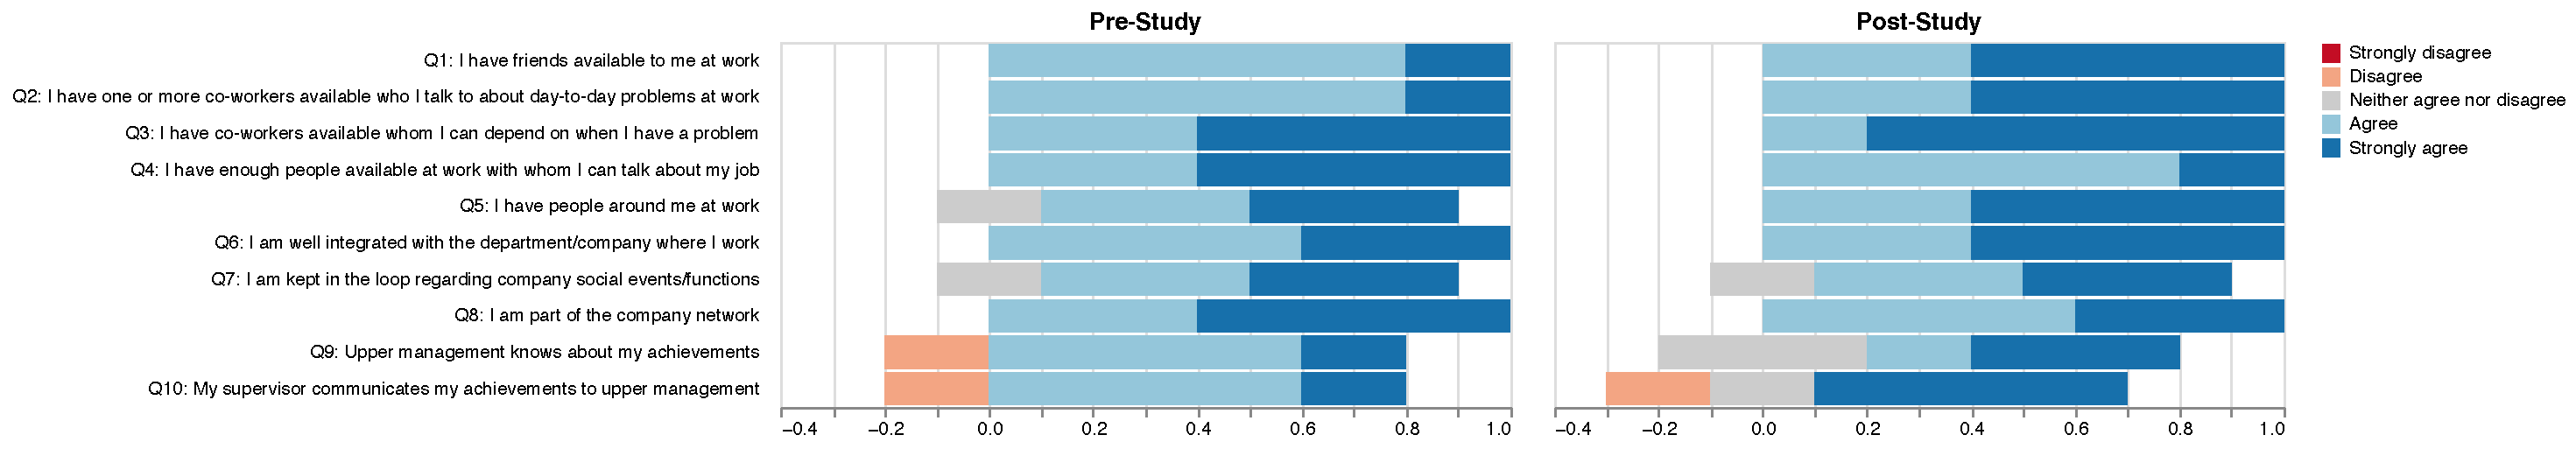
\includegraphics[width=\linewidth]{plots/workplace_isolation_likert.pdf}
    \caption{Results from the workplace isolation questionnaire, pre-study vs. post-study}
    \label{fig:workplace_isolation}
\end{figure}

In \autoref{fig:workplace_isolation}, we see a slight trend toward more \enquote{strongly agree} for questions 1-3, 5, 6, 9, and 10, indicating a decrease in feelings of isolation at work. However, some responses also slightly worsened, namely Q4 and Q8. Despite the results indicating improvement in Q9 and Q10, we cannot assume that these results are effects attributable to the use of AmbientTeams for two reasons. First, the content discussed within and triggered by AmbientTeams was not work-related. Second, due to the study's small size, there was no control group, so a comparison between the two questionnaire results is highly speculative. Nonetheless, as in this study, the questionnaire could be an excellent supplement for a more extensive study in the future to provide a more accurate statement of perceptions of isolation in the workplace. We see it as a valuable complement to the semi-structured interview and are optimistic about the potential of AmbientTeams to reduce feelings of workplace isolation in knowledge work teams.


\chapter{Future Directions}
\label{chapter:future_directions}

\section{Study Needed}
bias towards a young company culture -> young people might be more open for sharing moods -> interviews

% - P163: "sometimes you have this barrier to share the mood, so you have to establish this culture in the team, that it becomes a normal thing that everyone shares their angry or sad mood."

\section{Better Integration with Established Tools}
To increase the use and usage of AmbientTeams, participants Pxxx, Pxxx, and Pxxx all mentioned that a single tool would increase the likelihood and time they would use our mood-based micro-blogging approach.

\begin{displayquote}
    I think it would be good if AT could be integrated into Teams because if you have one tool, then you would use it more often. -P163
\end{displayquote}

\section{Self-Reflection}

\section{Task-Sharing}


Generally, x/y said that they would continue using it. X would continue using it if xyz was changed.
\chapter{Conclusion}
\label{chapter:conclusion}
After identifying the social challenges posed by remote work, AmbientTeams was developed to help knowledge workers address these issues, focusing on three main concepts: minimal design, focus on people and their well-being (via mood-based micro-blogging), and spontaneous interactions.

Complementing our initial research efforts, the interviews confirmed that there seems to be a need for an informal way of sharing information within knowledge work teams. Our approach aimed to help alleviate feelings of isolation in the workplace and communicate current social states with the team. The resulting research prototype, AmbientTeams, was used by a team consisting of five knowledge workers for five days. The usability questionnaire and interviews indicated that AmbientTeams was easy and intuitive to use, with the mood-sharing functionality being the most popular among participants. We then discussed the broader effects of AmbientTeams. We found that it 1) helped knowledge workers be aware of each other's moods and availability status, 2) got to know each other better, 3) enabled communication outside of AmbientTeams, and 4) spurred self-reflection on one's moods.

Further, we found that participants would reject automatic mood detection requiring constant camera access due to confidential data and privacy concerns. Nonetheless, other interesting directions for AmbientTeams were found and discussed. Possibilities to pursue in the future include focusing exclusively on the asynchronous exchange aspect and better integration with existing communication platforms.

\begin{appendices}
    \chapter{Consent Form}
\label{chapter:consent_form}

\begin{figure}[h]
    \centering
    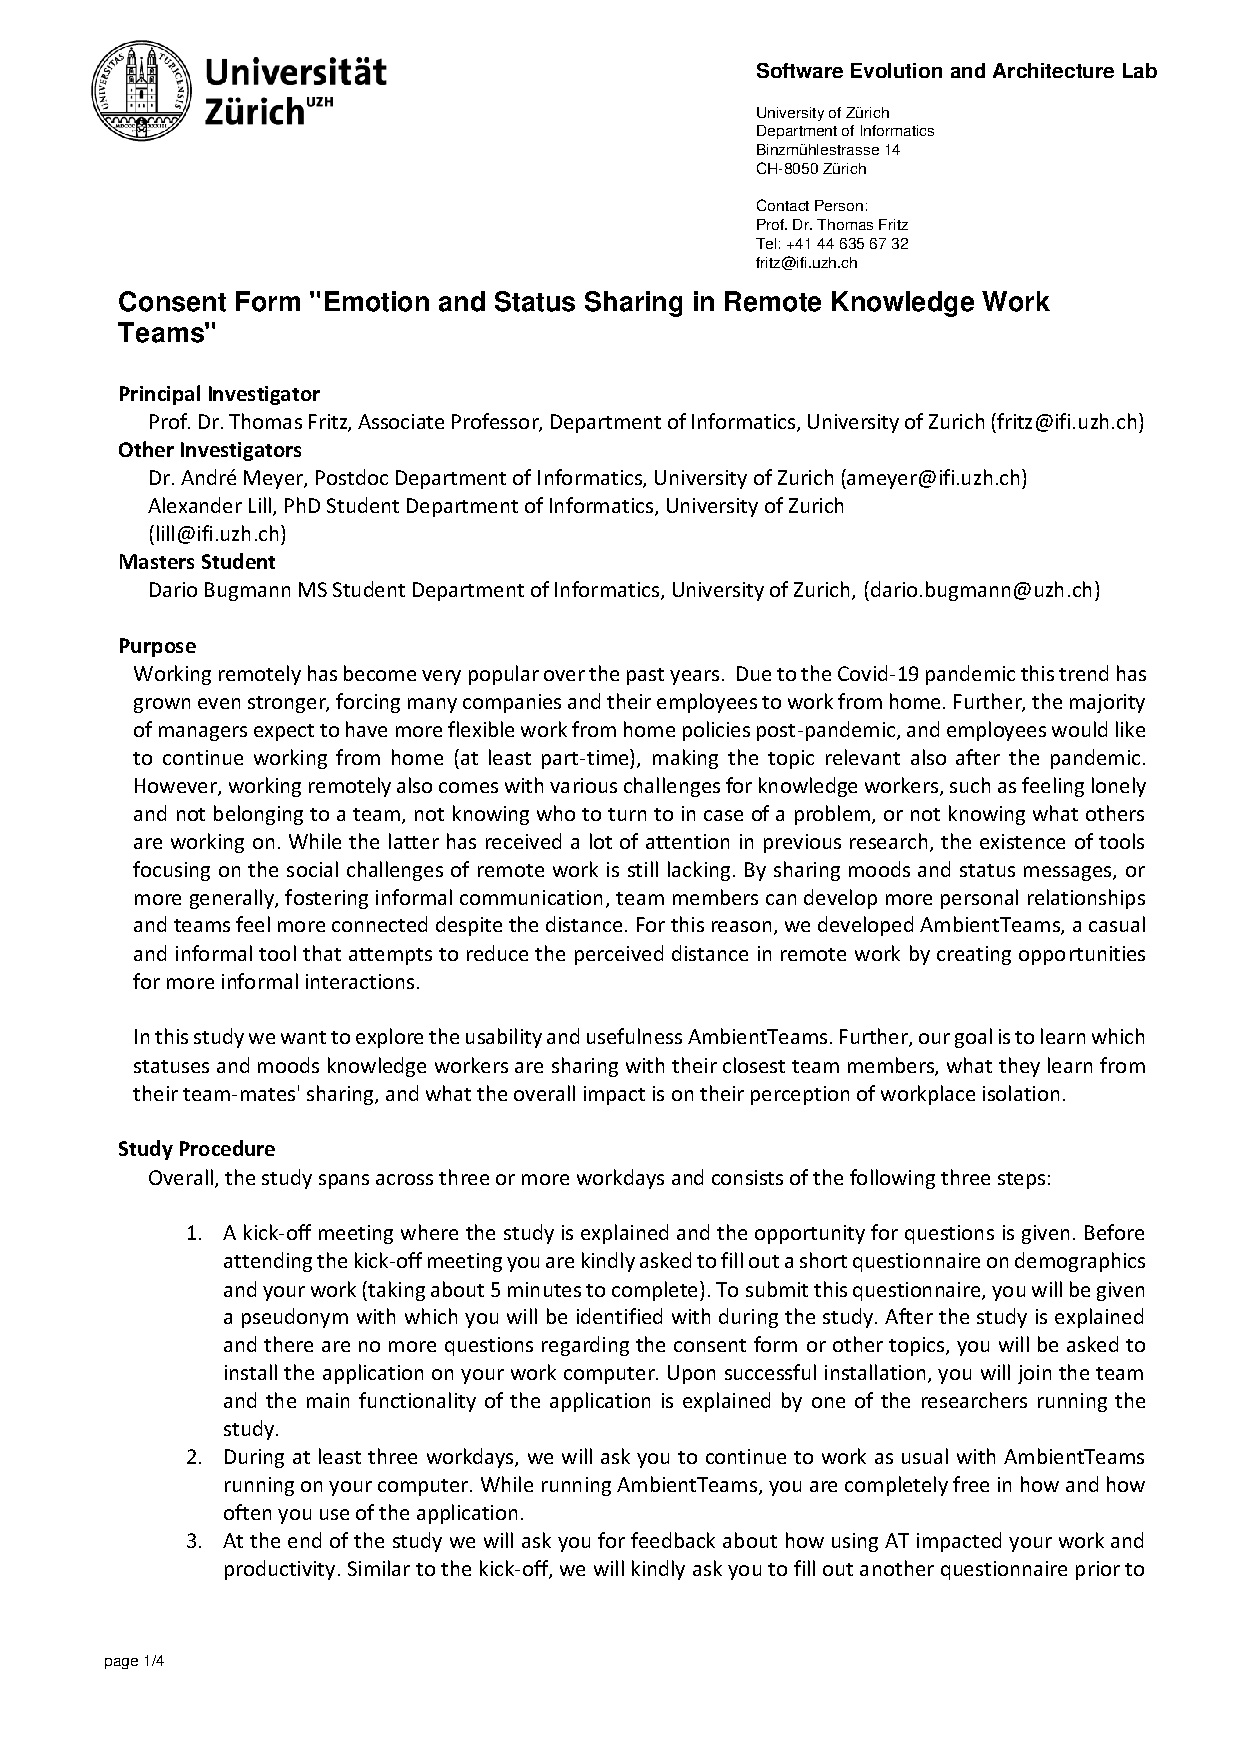
\includegraphics[width=\linewidth, page=1]{./documents/consent_form.pdf}
\end{figure}

\begin{figure}[h]
    \centering
    \includegraphics[width=\linewidth, page=2]{./documents/consent_form.pdf}
\end{figure}

\begin{figure}[h]
    \centering
    \includegraphics[width=\linewidth, page=3]{./documents/consent_form.pdf}
\end{figure}

\begin{figure}[h]
    \centering
    \includegraphics[width=\linewidth, page=4]{./documents/consent_form.pdf}
\end{figure}

\chapter{Study Instructions}
\label{chapter:study_instructions}

\begin{figure}[h]
    \centering
    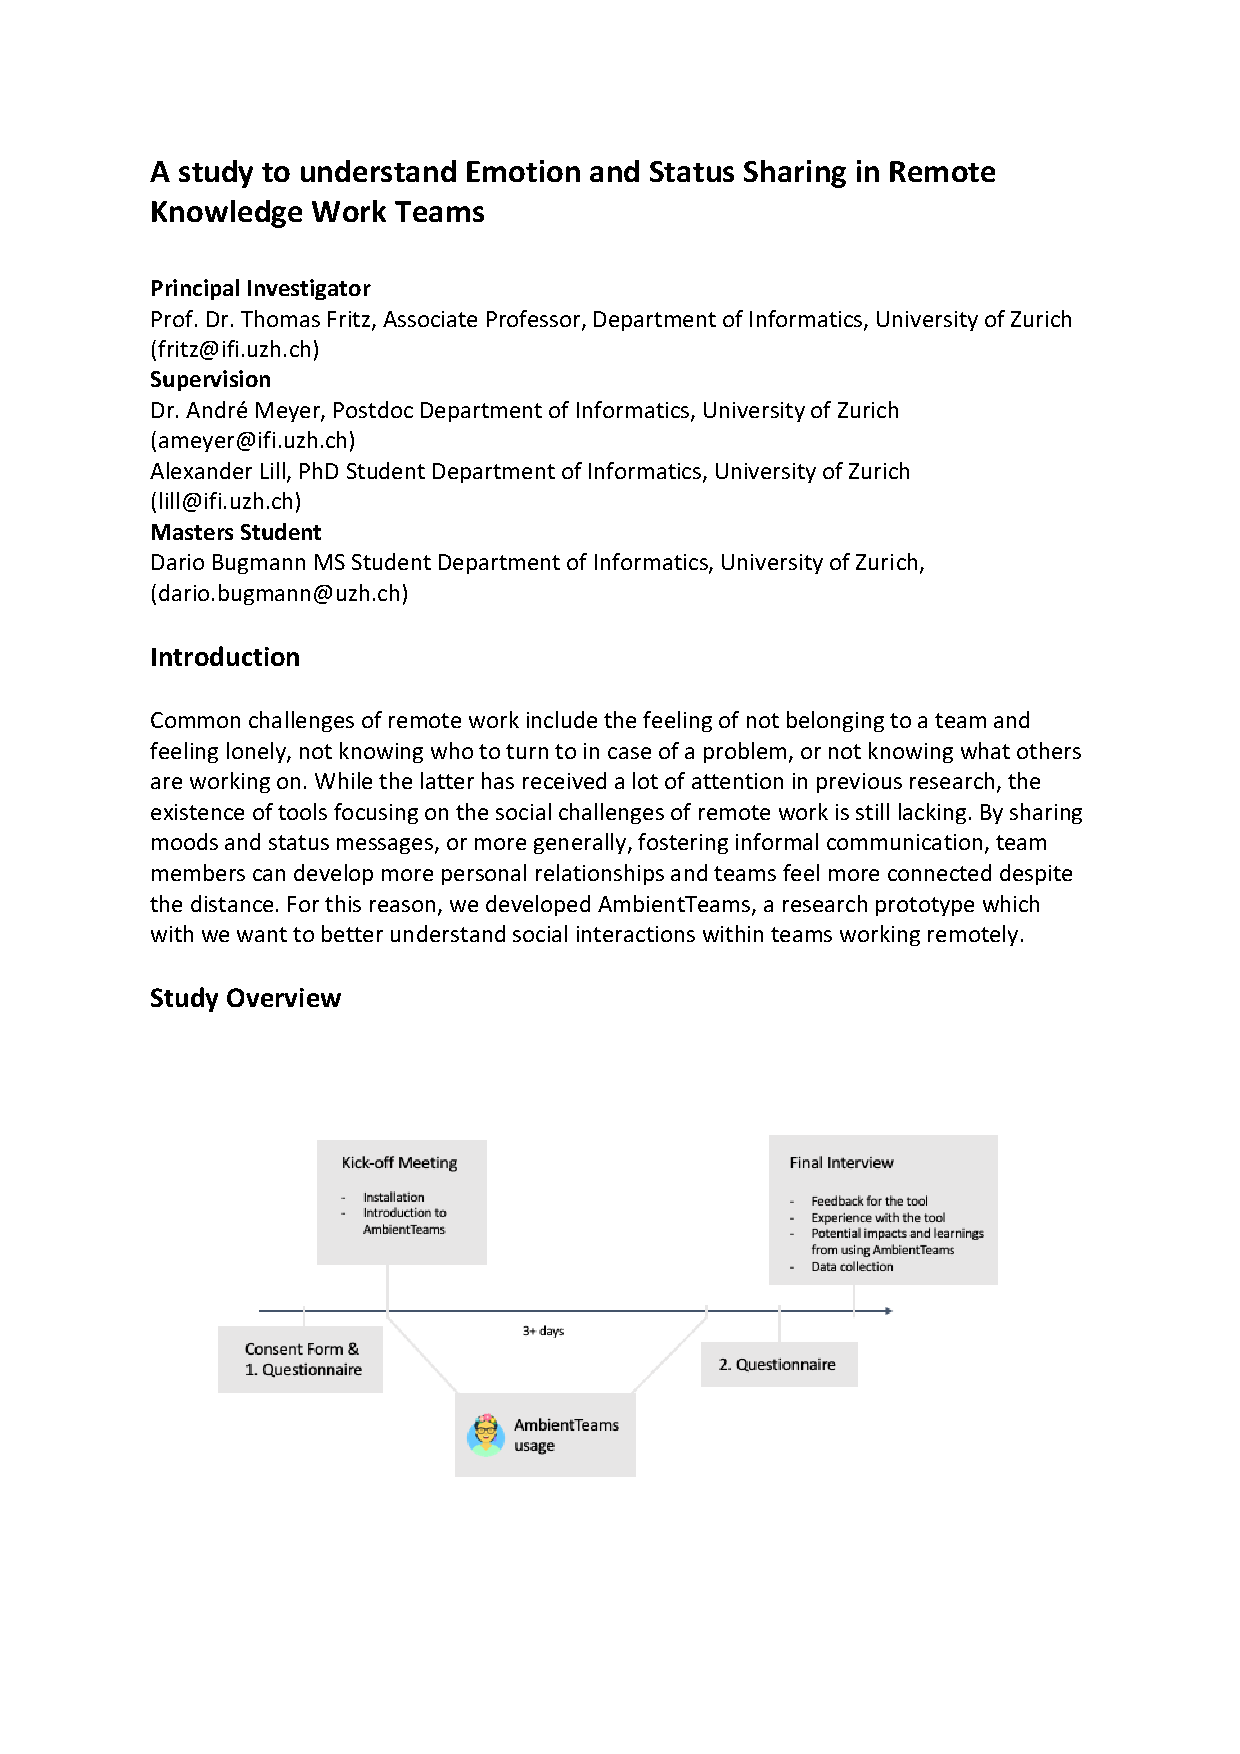
\includegraphics[width=\linewidth, page=1]{./documents/study_instructions.pdf}
\end{figure}

\begin{figure}[h]
    \centering
    \includegraphics[width=\linewidth, page=2]{./documents/study_instructions.pdf}
\end{figure}

\begin{figure}[h]
    \centering
    \includegraphics[width=\linewidth, page=3]{./documents/study_instructions.pdf}
\end{figure}

\begin{figure}[h]
    \centering
    \includegraphics[width=\linewidth, page=4]{./documents/study_instructions.pdf}
\end{figure}

\chapter{Pre-Study Questionnaire}
\label{chapter:prestudy_questionnaire}

\begin{figure}[h]
    \centering
    \includegraphics[width=\linewidth, page=1]{./documents/Prestudy_Questionnaire.pdf}
\end{figure}

\begin{figure}[h]
    \centering
    \includegraphics[width=\linewidth, page=2]{./documents/Prestudy_Questionnaire.pdf}
\end{figure}

\chapter{Post-Study Questionnaire}
\label{chapter:poststudy_questionnaire}

\begin{figure}[h]
    \centering
    \includegraphics[width=\linewidth, page=1]{./documents/poststudy_Questionnaire.pdf}
\end{figure}

\begin{figure}[h]
    \centering
    \includegraphics[width=\linewidth, page=2]{./documents/Poststudy_Questionnaire.pdf}
\end{figure}

\chapter{Semi-Structured Interview Guide}
\label{chapter:interview_guide}
\begin{figure}[h]
    \centering
    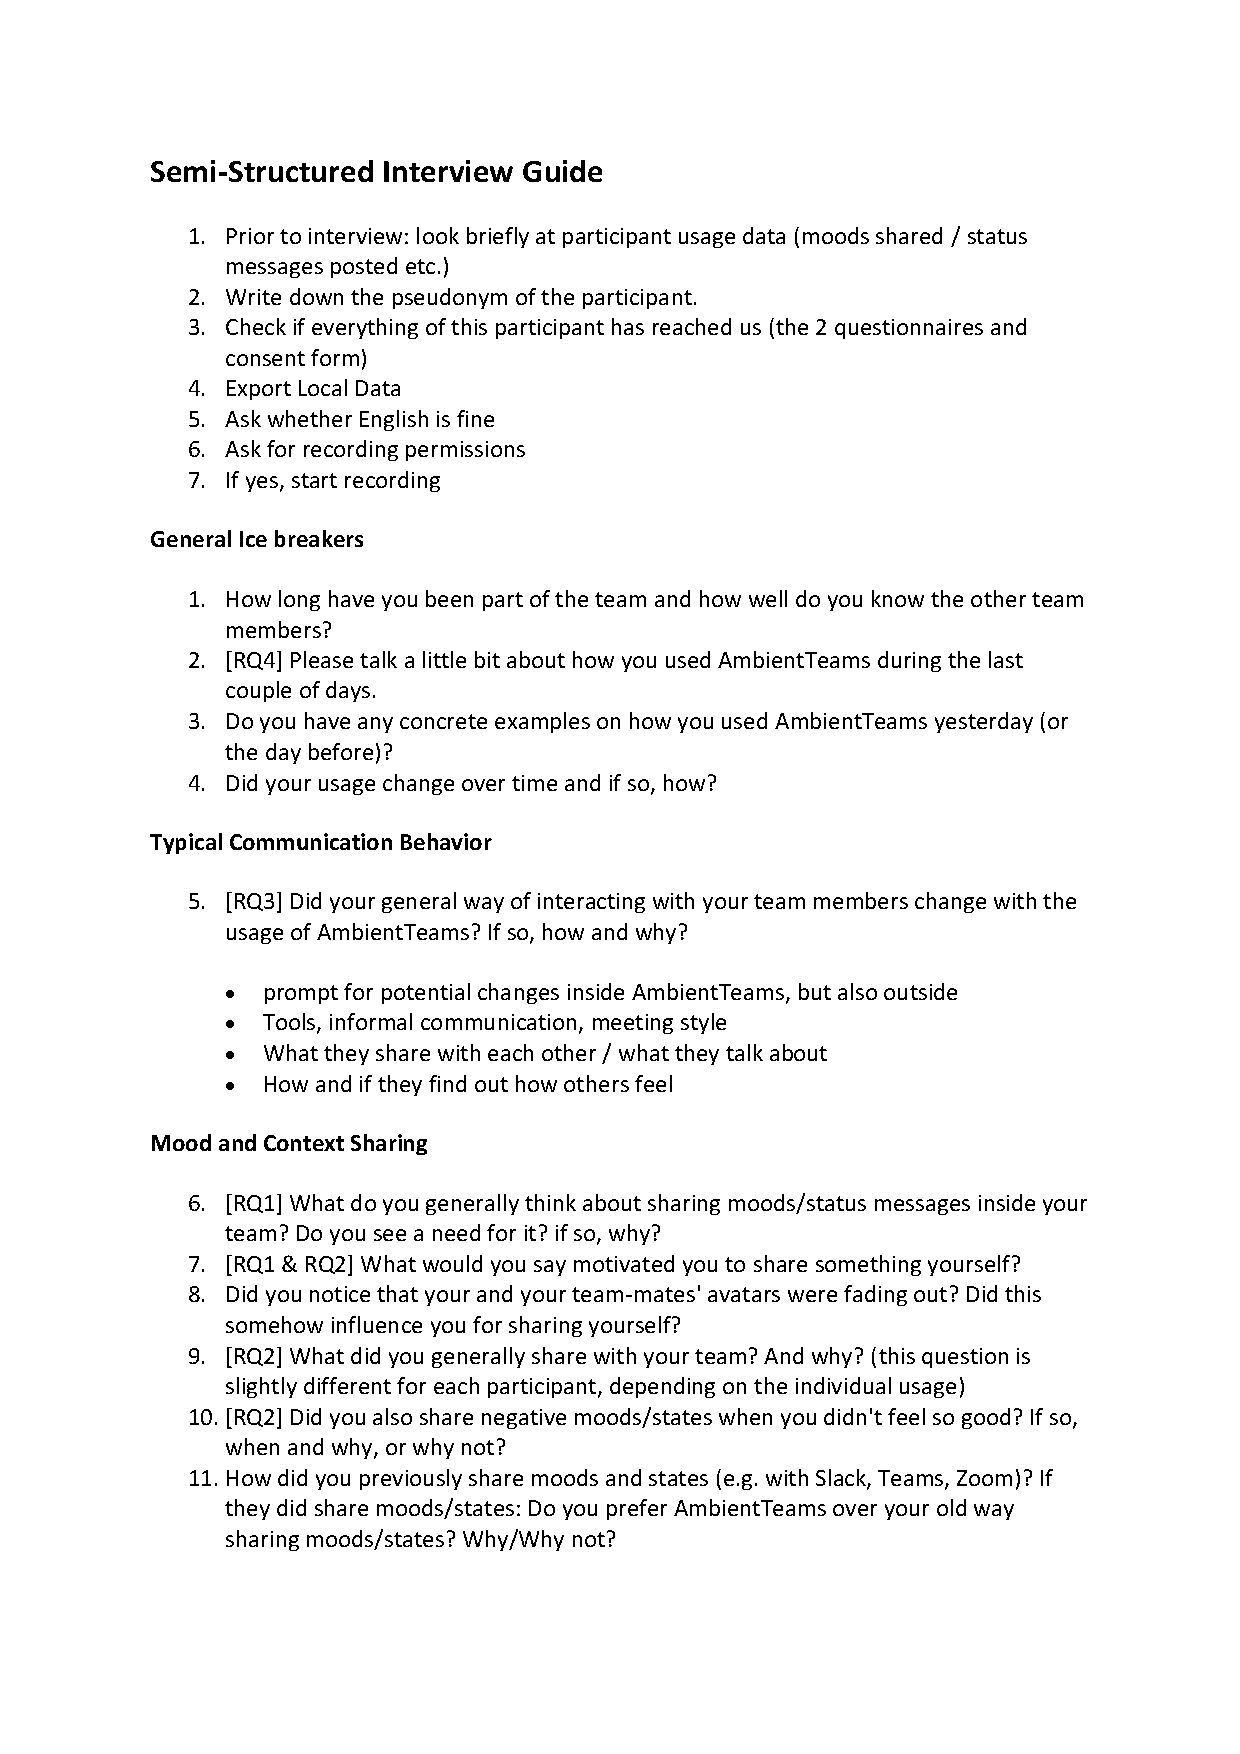
\includegraphics[width=\linewidth, page=1]{./documents/Semi-Structured Interview Guide.pdf}
\end{figure}

\begin{figure}[h]
    \centering
    \includegraphics[width=\linewidth, page=2]{./documents/Semi-Structured Interview Guide.pdf}
\end{figure}

\begin{figure}[h]
    \centering
    \includegraphics[width=\linewidth, page=3]{./documents/Semi-Structured Interview Guide.pdf}
\end{figure}
\end{appendices}


\backmatter
\printbibliography

\end{document}
